\documentclass{scrartcl}

\usepackage{ucs}
\usepackage[utf8x]{inputenc}
\usepackage[ngerman]{babel}
\usepackage[hidelinks]{hyperref}
\usepackage{graphicx}
\usepackage{amsmath}
\usepackage{amssymb}
\usepackage{color}
\usepackage{listings}

\definecolor{pblue}{rgb}{0.13,0.13,1}
\definecolor{pgreen}{rgb}{0,0.5,0}
\definecolor{pred}{rgb}{0.9,0,0}
\definecolor{pgrey}{rgb}{0.46,0.45,0.48}
\definecolor{light-gray}{gray}{0.95}

\lstset{
	backgroundcolor=\color{light-gray},
	language=Java,
	showspaces=false,
	showtabs=false,
	breaklines=true,
	showstringspaces=false,
	breakatwhitespace=true,
	commentstyle=\color{pgreen},
	keywordstyle=\color{pblue},
	stringstyle=\color{pred},
	basicstyle=\ttfamily,
	moredelim=[il][\textcolor{pgrey}]{$$},
	moredelim=[is][\textcolor{pgrey}]{\%\%}{\%\%}
}

\setlength\parindent{0pt}

\title{Grafikprogrammierung 1 \\ Zusammenfassung}
\author{Thomas Mohr}
\date{}

\begin{document}
\maketitle
\pagebreak
\tableofcontents{}

\section{GUIs}

\subsection{Grafische Benutzerschnittstellen}

\subsubsection{Gestaltpsychologie}

\begin{tabular}{|c|c|c|}
	\hline Gesetz der Nähe & \parbox[c][4cm]{5cm}{Nahe beieinander platzierte Objekte gehören zusammen} & \raisebox{-.5\height}{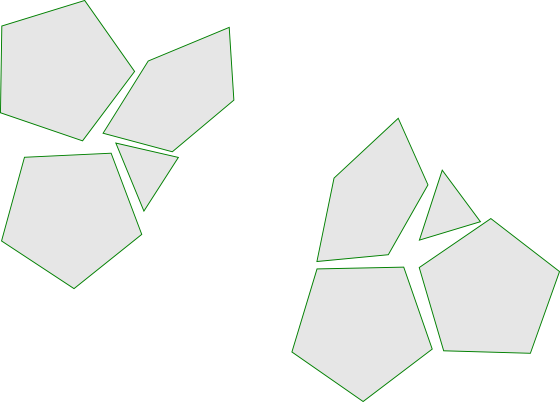
\includegraphics[scale=0.25]{figures/gestalt_proximity.png}}  \\ 
	\hline Gesetz der Ähnlichkeit & \parbox[c][4cm]{5cm}{Objekte mit der gleichen Farbe, Form, Größe, Orientierung, etc. gehören zusammen} & \raisebox{-.5\height}{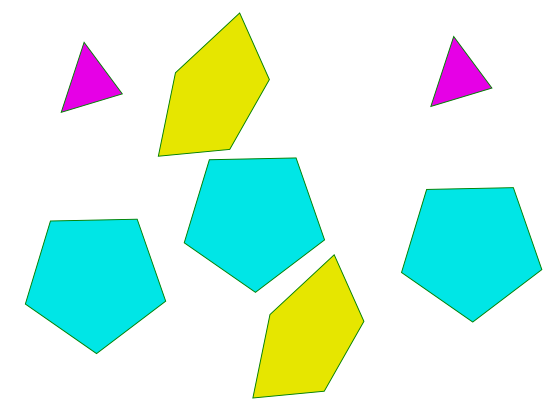
\includegraphics[scale=0.25]{figures/gestalt_similarity.png}}  \\ 
	\hline Gesetz der einfachen Gestalt & \parbox[c][4cm]{5cm}{Komponenten werden gruppiert, wenn sie gemeinsam eine einfache Form ergeben} & \raisebox{-.5\height}{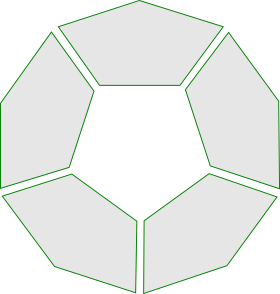
\includegraphics[scale=0.25]{figures/gestalt_closure.png}}  \\ 
	\hline Gesetz der Kontinuität & \parbox[c][4cm]{5cm}{Kleine Komponenten werden zu größeren Objekten gruppiert, wenn Linien/Kurven kontinuierlich fortgesetzt werden können} & \raisebox{-.5\height}{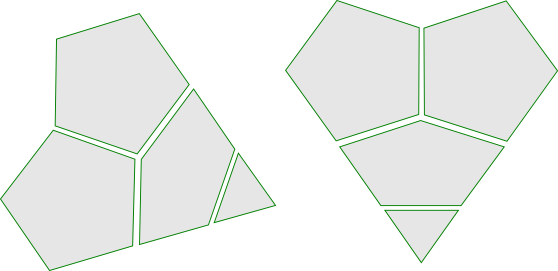
\includegraphics[scale=0.25]{figures/gestalt_continuity.png}}  \\ 
	\hline 
\end{tabular}

\subsubsection{Acht goldene Regeln für gutes GUI-Design}

\begin{enumerate}
	\item Strebe nach Konsistenz
	\item Erlaube geübten Nutzern, Tastenkürzel zu verwenden
	\item Biete dem Nutzer informative Rückmeldungen an
	\item Entwerfe abgeschlossene Dialoge, die einen Start und ein Ende haben
	\item Biete einfache Fehlerbehandlung
	\item Erlaube die Umkehrung von Aktionen (Undo)
	\item Gib dem Nutzer das Gefühl, die Anwendung zu kontrollieren
	\item Verringere die Informationen, die der Nutzer im Kurzzeitgedächtnis behalten muss
\end{enumerate}

\subsection{GUIs mit Java}

\subsubsection{Java Foundation Classes (JFC)}

\begin{tabular}{|c|c|}
	\hline \textbf{API} & \textbf{Funktion} \\ 
	\hline Abstract Window Toolkit & Basisklassen für GUI-Komponenten, Events und Layouts \\ 
	\hline Swing & GUI-Komponenten, veränderbarer Look-and-Feel \\ 
	\hline Java 2D & Zeichnen von 2D-Elementen \\ 
	\hline Java Accessibility & Unterstützungstechnologien z.B. für Mensch mit Sehbehinderung \\ 
	\hline Data Transfer & Cut-and-Paste, Drag-and-Drop \\ 
	\hline 
\end{tabular}

\subsubsection{Ereignisverarbeitung}

Der Event Dispatching Thread (EDT) läuft im Hintergrund und arbeitet die Ereignisse aller Ereignisquellen nacheinander ab.

\subsubsection{Layout-Manager}

\begin{itemize}
	\item BorderLayout
	\begin{itemize}
		\item Der BorderLayout-Manager ist der voreingestellte Standard für viele Fenster, z.B. JFrame
		\item Das Layout unterteilt das Fenster in 5 Bereiche: Norden, Osten, Süden, Westen und Zentrum
	\end{itemize}
	\item GridLayout
	\begin{itemize}
		\item Der GridLayout-Manager ordnet die Komponenten auf einem regulären Gitter an
		\item Die Komponenten versuchen, ihre zugewiesene Gitterzelle zu füllen
	\end{itemize}
	\item SpringLayout
	\begin{itemize}
		\item Der SpringLayout-Manager ist relativ kompliziert zu handhaben und ist eigentlich für die Verwendung mit visuellen GUI-Editoren konzipiert
		\item Er ist eine gute Wahl, wenn es z.B. um die Erstellung eines Formulars geht
	\end{itemize}
\end{itemize}

\subsection{GUIs mit Java (Android)}

\subsubsection{Lebenszyklus einer Activity}

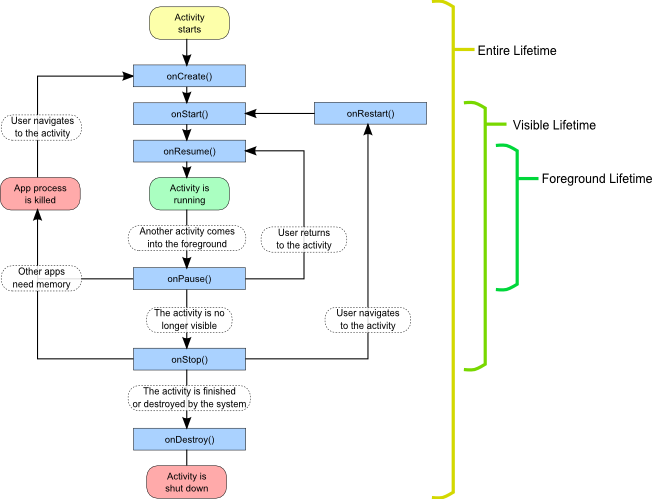
\includegraphics[scale=0.9]{figures/activity_lifecycle.png}

\subsubsection{Activity Instance State}

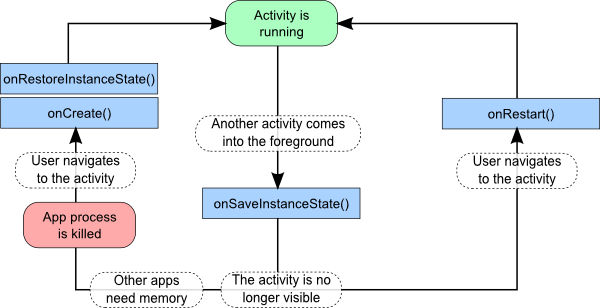
\includegraphics[scale=1]{figures/activity_instancestate.png}

\subsection{GUIs mit C++ und Qt}

TODO

\section{2D Objekte}

\subsection{Vektor- und Rastergrafik}

\subsubsection{Vektorgrafik}

\begin{itemize}
	\item In der Vektorgrafik werden die Objekte durch Kombination von Basisobjekten (wie z.B. Linie, Rechteck, Kreis, Dreieck, Polygon) beschrieben.
	\item  Die Koordinaten ($x$-Koordinate und $y$-Koordinate) beginnen in der linken oberen Ecke.
	\item  Der Vorteil von Vektorgrafiken ist, dass sie verlustfrei skaliert werden können.
\end{itemize}

\subsubsection{Rastergrafik}

\begin{itemize}
	\item Die heutigen Bildschirme stellen einzelene Bildelemente dar (Pixel = ''Picture Elements''), die auf einem festen Raster angeordnet sind.
	\item Rastergrafiken besitzen einen Farbwert für jedes Pixel ihres Rasters. Sind sind daher vollständig definiert durch:
	\begin{itemize}
		\item Bildbreite: Anzahl der Pixel in $x$-Richtung
		\item Bildhöhe: Anzahl der Pixel in $y$-Richtung
		\item und einem Datenfeld mit (Breite $\cdot$ Höhe) Farbwerten
	\end{itemize}
	\item  Die Koordinaten ($x$-Koordinate und $y$-Koordinate) beginnen ebenfalls in der linken oberen Ecke.
\end{itemize}

\begin{itemize}
	\item Vorteile Rastergrafik
	\begin{itemize}
		\item Sehr geeignet für komplexe Szenen mit unregelmäßigen Formen oder vielen Farben
		\item Speicherbedarf ist unabhängig von der Szenenkomplexität
		\item Direkte Darstellung auf heutigen Bildschirmen
	\end{itemize}
	\item Nachteile Rastergrafik
	\begin{itemize}
		\item Bei der Darstellung sehr einfacher Objekte ist der Speicherbedarf im Vergleich zu einer Vektorgrafik höher
		\item Bei starker Vergrößerung werden einzelne Pixel erkennbar
		\item Dieser Effekt wird auch Treppeneffekt oder Aliasing genannt
	\end{itemize}
\end{itemize}

\subsection{Rasterkonvertierung}

\subsubsection{Geradengleichung aus zwei Punkten}

\begin{equation}
	\begin{split}
	\frac{y - y_0}{x - x_0} &= \frac{y_1 - y_0}{x_1 - x_0} \\
	y - y_0 &= \underbrace{\frac{y_1 - y_0}{x_1 -x_0}}_m (x - x_0) \\
	y &= m(x- x_0) + y_0 \\
	y &= mx \underbrace{-mx_0 + y_0}_b \\
	y &= mx + b
	\end{split}
\end{equation}

\subsubsection{Mittelpunktalgorithmus}

Beobachtung von Bresenham (1965): \\

\begin{itemize}
	\item Wenn die (for-) Schleife in $x$-Richtung läuft und ein Pixel gezeíchnet wurde, gibt es nur zwei Optionen für das nächste Pixel:
	\begin{itemize}
		\item Keine Erhöhung $\rightarrow$ nächstes Pixel $(x + 1, y)$
		\item Erhöhung um 1 $\rightarrow$ nächstes Pixel $(x + 1, y + 1)$
	\end{itemize}
	\item Die Entscheidung, welcher Fall vorliegt, kann durch Betrachtung des Mittelpunkts \\
$(x + 1, y + 0.5)$ getroffen werden.
	\begin{itemize}
		\item Gerade unter Mittelpunkt $\rightarrow$ Keine Erhöhung
		\item Gerade über Mittelpunkt $\rightarrow$ Erhöhung um 1
	\end{itemize}
	\begin{equation}
		\begin{split}
			\frac{y - y_0}{x - x_0} &= \frac{y_1 - y_0}{x_1 - x_0} \\
	(y - y_0) \underbrace{(x_1 - x_0)}_{\Delta_x} &= \underbrace{(y_1 - y_0)}_{\Delta_y} (x - x_0) \\
			(y - y_0) \Delta_x &= \Delta_y (x - x_0) \\
			0 &= \Delta_y x - \Delta_x y - \Delta_y x_0 + \Delta_x y_0 \\
			g(x,y) &= \underbrace{\Delta_y}_a x \underbrace{-\Delta_x}_b y + \underbrace{\Delta_x y_0 - \Delta_y x_0}_c \\
			g(x,y) &= ax + by + c
		\end{split}
	\end{equation}
	\item Implizite Geradengleichung
	\begin{itemize}
		\item Wenn g(x,y) = 0 $\rightarrow$ Punkt auf der Geraden
		\item Wenn g(x,y) $<$ 0 $\rightarrow$ Punkt unterhalb der Geraden
		\item Wenn g(x,y) $>$ 0 $\rightarrow$ Punkt oberhalb der Geraden
	\end{itemize}
	\item Mittelpunktalgorithmus
	\begin{itemize}
		\item Wenn $g(x + 1, y + 0.5) \leq 0 \rightarrow$ Keine Erhöhung
		\item Wenn $g(x + 1, y + 0.5) > 0 \rightarrow$ Erhöhung um 1
	\end{itemize}
\end{itemize}

\subsubsection{Rasterkonvertierung von Kreisen}

\begin{itemize}
	\item Implizite Gleichung für einen Kreis mit Radius $r: g(x,y) = x^2 + y^2 - r^2$
	\begin{itemize}
		\item Wenn $g(x,y) = 0 \rightarrow$ Punkt auf dem Kreis
		\item Wenn $g(x,y) < 0 \rightarrow$ Punkt innerhalb des Kreises
		\item Wenn $g(x,y) > 0 \rightarrow$ Punkt außerhalb des Kreises
	\end{itemize}
\end{itemize}

\begin{itemize}
	\item Das Vorgehen zum Zeichnen von Kreisen ist sehr ähnlich zu dem für Linien.
	\item Aufgrund der Symmetrie muss allerdings nur eich Achtel des Kreisumfangs berechnet werden und die anderen Pixel können kopiert werden.
\end{itemize}

\begin{itemize}
	\item Der Mittelpunktalgorithmus für Kreise ist sehr ähnlich dem für Linien. Er verwendet die implizite Kreisgleichung und wertet die Position des nächsten Pixel-Mittelpunkts $(x + 1, y - 0.5)$ aus.
	\item Es gilt $x_{init} = 0, y_{init} = r$.
	\item Mittelpunktalgorithmus
	\begin{itemize}
		\item Wenn $g(x + 1, y - 0.5) \leq 0 \rightarrow$ Keine Reduktion von y
		\item Wenn $g(x + 1, y - 0.5) > 0 \rightarrow$ Reduktion von y um 1
	\end{itemize}
\end{itemize}

\subsubsection{Rasterkonvertierung von Polygonen (Scanline-Algorithmus)}

\begin{itemize}
	\item Beim Scanline-Algorithmus wird das Pixelraster zeilenweise durchlaufen.
	\item Schritt 1: Für jede Zeile werden die Schnittpunkte mit den Polygonkanten berechnet.
	\item Schritt 2: Diese Schnittpunkte werden nach ihrer x-Koordinate aufsteigend sortiert.
	\item Schritt 3: Durchlaufe die Pixel der Scanline beginnend bei $x = 0$. Zeichne Pixel nur, wenn die Parität der bisher durchlaufenen Schnittpunkte ungerade ist (Regel der ungeraden Parität).
\end{itemize}

\subsubsection{Rasterkonvertierung von Pineda}

\begin{itemize}
	\item Ein einfacher, parallelisierbarer Algorithmus für die Rasterkonvertierung von konvexen Polygonen wurde 1988 von Pindea vorgeschlagen.
	\item Die grundlegende Idee: Verwende die Hessische Normalform der Geraden, die die Kanten des Polygons bilden, um zu entscheiden, ob ein Pixel innerhalb oder außerhalb des Polygons liegt.
	\item Dazu wird angenommen, dass die Kanten das Polygon im Uhrzeigersinn umlaufen. Liegt ein Pixel rechts von jeder Gerade, ist es innerhalb.
\end{itemize}

TODO Normale und Hessische Normalform

\subsection{Clipping}

\subsubsection{Clipping von Liniensegmenten}

\begin{itemize}
	\item Clipping von Liniensegmenten an einem rechteckigen Fenster (an konvexem Objekt)
	\item Unterteilung einer Geraden in sichtbare und unsichtbare Teile
	\item Vektoren deren beide Endpunkte oberhalb, unterhalb, rechts oder links des Fensters liegen, sind völlig unsichtbar $\rightarrow$ Vektoren (Linien) werden aussortiert
\end{itemize}

TODO ergänzen

\section{OpenGL Pipeline}

\subsection{Definition}

\begin{itemize}
	\item Die Grafikbefehle werden vom Grafiktreiber umgesetzt und sind damit unabhängig von
	\begin{itemize}
		\item der Grafikkarten-Hardware
		\item dem Betriebssystem
		\item dem verwendeten Fenster-Manager
	\end{itemize}
	\item Grafikbefehle sind einigermaßen hardwarenah und ausreichend, um die Kernfunktionalität
	\item Verschiedene Bibiliotheken basieren auf OpenGL und erlauben Programmierung auf höherem Abstraktionsniveau
\end{itemize}

\subsection{OpenGL als Zustandsmaschine}

\begin{itemize}
	\item Beim Zeichnen befindet sich OpenGL in bestimmten Zuständen, die das Verhalten und die Ausgabe beeinflussen
	\item Z.B. setzt der Befehl $glColor(\ldots)$ die aktuelle Zeichenfarbe
	\item Dieser Zustand bleibt gesetzt bis er durch einen anderen Grafikbefehl verändert wird, also z.B. bis zum nächsten Aufruf von $glColor(\ldots)$
\end{itemize}

\subsection{OpenGL-Pipeline}

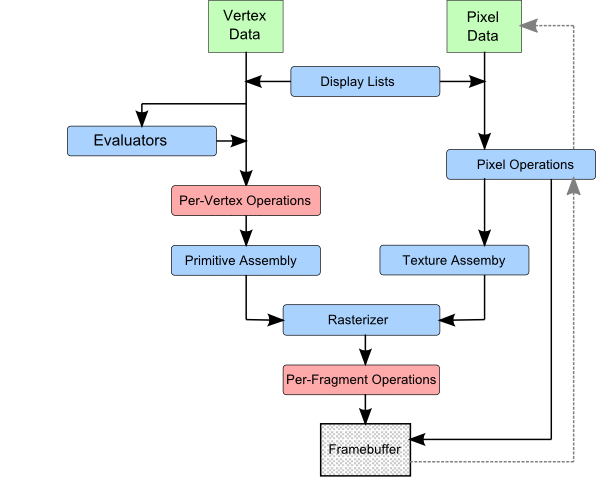
\includegraphics[scale=1]{figures/openglpipeline_animate0.png}

\begin{enumerate}
	\item Frambuffer
	\begin{itemize}
		\item Der Framebuffer ist eine Rastergrafik, d.h. er hat eine bestimmte Breite und Höhe und enthält Pixel, die auf einem festen Raster angeordnet sind.
	\end{itemize}
	\item Vertex Daten
	\begin{itemize}
		\item Ein Vertex ist ein Stützpunkt eines Grafikobjekts, z.B. Linie, Dreieck, Polygon, etc.
		\item Mit $glVertex(\ldots)$ werden die Stützpunkte einzeln übergeben.
	\end{itemize}
	\item Evaluators
	\begin{itemize}
		\item Anstatt durch Vertex Daten können Grafikobjekte auch durch parametrische Beschreibungen definiert werden, z.B. durch Kontrollpunkte von parametrischen Kurven oder Oberflächen.
		\item Evaluatoren wandeln die parametrische Beschreibung in Vertex Daten um, so dass letztendlich im Rest der Pipeline immer mit Vertex Daten gearbeitet werden kann.
	\end{itemize}
	\item Per-Vertex Daten
	\begin{itemize}
		\item In diesem Schritt werden für jeden Vertex eine Reihe von Operationen durchgeführt.
		\item Bei Verwendung der Fixed-Function Pipeline sind dies z.B.
		\begin{itemize}
			\item Die Transformationen der Stützpunkte vom globalen Welt- ins Kamerakoordinatensystem und die Projektion in die Kamerabildebene.
			\item Generierung von Normalen oder Texturkoordinaten und deren Transformation.
			\item Berechnung einer Vertex Farbe bei gegebener Beleuchtung.
		\end{itemize}
		\item Bei der Verwendung von Shadern, wird dieser Schritt mittels eines so genannten Vertex-Shaders implementiert.
	\end{itemize}
	\item Zusammenbauen von Primitiven (Primitive Assembly)
	\begin{itemize}
		\item Beim Zusammenbauen von Primitiven werden die Vertex Daten unterschiedlich verwendet. Dies ist abhängig von dem Argument von $glBegin(\ldots)$.
		\item In diesem Schritt werden ebenfalls 3D-Clipping Operationen durchgeführt. Durch das Clipping können zusätzliche Stützpunkte erzeugt werden.
		\item Danach wird eine perspektivische Division durchgeführt, die die persepektivische 2D-Abbildung der Objekte realisiert.
		\item Nicht sichtbare Primitive können entfernt werden.
		\item Abschließend werden die 2D-Koordinaten entsprechend der gewählten Bildauflösung und -position skaliert und/oder verschoben.
		\item Die erzeugten Primitive kennen nun ihre 2D-Koordinaten (reele Zahlen) im Framebuffer und werden an den 2D-Rasterisierer übergeben.
	\end{itemize}
	\item Pixel Daten
	\begin{itemize}
		\item Mit OpenGL können ebenfalls Rastergrafiken verarbeitet werden.
		\item Außerdem werden Rasterbilder häufig als Texturen (''Farbtapete'') verwendet.
		\item Es ist ebenfalls möglich, ein Bild aus de Framebuffer als Eingabe für einen zweiten Rendering-Durchgang zu verwenden.
		\item Pixel Daten werden vom Hauptspeicher des Computers in ein bestimmtes OpenGL-Speicherformat konvertiert
		\item Es können Bildmanipulationen durchgeführt werden, wie Vergrößern, Verkleinernm, Umdrehen des Bildes, Farbwerte manipulieren, Filter anwenden, etc.
		\item Viele dieser Operationen sind Teil der Fixed-Function Pipeline und werden heutzutage in der Regel stattdessen durch Textur- und Framebuffer-Objekte realisiert.
	\end{itemize}
	\item Zusammenbauen von Texturen (Texture Assembly)
	\begin{itemize}
		\item Pixel Daten können ebenfalls als Texturen verwendet werden.
		\item Texturen werden in Textur-Objekten gespeichert, die mit einer ID (Kennung) ausgestattet sind und so refernziert und wiederverwendet werden können.
		\item D.h. die Pixel müssen nur bei der Erzeugung der Textur vom Hauptspeicher des Computers auf den Grafikkartenspeicher transferiert werden und stehen anschließend dort zur Verfügung.
		\item Die Grafikkarten-Hardware unterstützt den schnellen Zugriff auf Texturen.
	\end{itemize}
	\item Rasterisierer
	\begin{itemize}
		\item Der Rasterisierer konvertiert die prozessierten Vertex- oder Pixel-Daten in so genannte Fragmente.
		\item Die Rasterkonvertierung wird auch auf modernen Grafikkarten (mit programmierbaren Shader-Einheiten) noch durch dedizierte Hardware realisiert.
		\item Jedes Fragment kennt seinen interpolierten Farbwert, Tiefenwert und evtl. seine Textur Koordinate.
	\end{itemize}
	\item Per-Fragment Operationen
	\begin{itemize}
		\item Bevor die Fragment-Daten als Pixelwerte im Framebuffer landen, werden noch eine Reihe von Operationen für jedes Fragment ausgeführt.
		\item Bei Verwendung der Fixed-Function Pipeline sind dies z.B.
		\begin{itemize}
			\item Texturierung
			\item Farbgenerierung oder -manipulation
			\item Nebelerzeugung (Fog)
		\end{itemize}
		\item Bei der Verwendung von Shadern, kann dieser Schritt mittels eines sogenannten Fragment-Shaders implementiert werden.
		\item Das resultierende Fragment durchläuft dann noch einige weitere (optionale) Verarbeitungsschritte bis die Information im Framebuffer landet:
		\begin{enumerate}
			\item Scissor-Test
			\item Alpha-Test
			\item Depth-Test
			\item Stencil-Test
			\item Blending
			\item Dithering
			\item Logische Operationen
		\end{enumerate}
	\end{itemize}
\end{enumerate}

\section{Objekttransformationen}

\subsection{2D Transformationen}

\begin{tabular}{|c|c|c|}
	\hline Transformationsart & Formel & Bild \\ 
	\hline 2D Translation & \parbox[c][4cm]{6cm}{$\widetilde{p} = (\frac{\widetilde{x}}{\widetilde{y}}) = (\frac{x + t_x}{y + t_y}) = p + (\frac{t_x}{t_y}) = p + t$} & \raisebox{-.5\height}{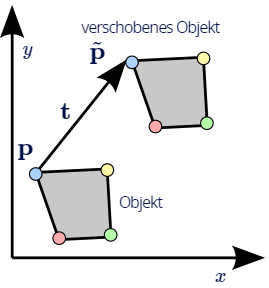
\includegraphics[scale=0.3]{figures/translation.png}} \\ 
	\hline 2D Skalierung & \parbox[c][6cm]{6cm}{Bei einer Vergrößerung des Objekts um den Faktor s gilt:
	\begin{equation}
		\widetilde{p} = (\frac{sx}{sy}) = sp
	\end{equation}
	Bzw. bei nicht gleichförmiger Skalierung in x- und y-Richtung:
	\begin{equation}
		\widetilde{p} = (\frac{s_x x}{s_y y}) = \begin{bmatrix}
	s_x & 0 \\
	0 & s_y
	\end{bmatrix}p
	\end{equation}		
	} & \raisebox{-.5\height}{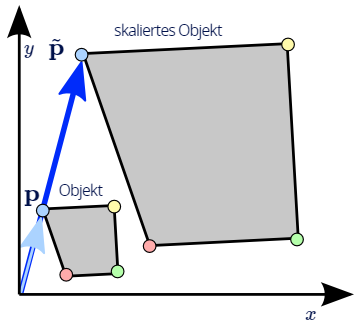
\includegraphics[scale=0.3]{figures/scale.png}} \\
	\hline 2D Rotation & \parbox[c][4cm]{6cm}{$\widetilde{b}_x = (\frac{\cos \alpha}{\sin \alpha}) \text{ und } \widetilde{b}_y = (\frac{-\sin \alpha}{\cos \alpha})$} & \raisebox{-.5\height}{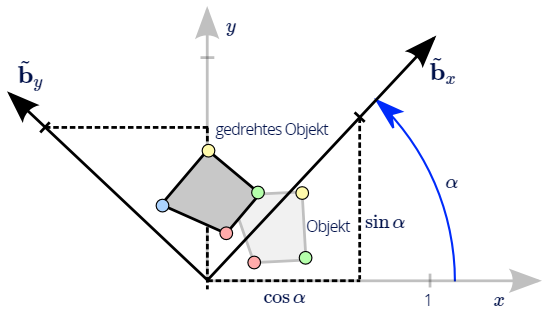
\includegraphics[scale=0.3]{figures/rotation.png}} \\
	\hline
\end{tabular} 

\subsubsection{2D Rotation}

Um ein Objekt zu drehen, können die gegebenen Objektkoordinaten von $p = (x,y)^\top$ im gedrehten Koordinatensystem abgetragen werden. Dann gilt für den gedrehten Punkt $\widetilde{p}$ im ursprünglichen Koordinatensystem: \\

\begin{equation}
	\begin{split}
	\widetilde{p} &= \widetilde{b}_x x + \widetilde{b}_y y \\
	&= (\frac{\cos \alpha}{\sin \alpha})x + (\frac{-\sin \alpha}{\cos \alpha})y \\
	&= \underbrace{[\widetilde{b}_x \widetilde{b}_y]}_R (\frac{x}{y}) \\
	&= \underbrace{\begin{bmatrix}
	\cos \alpha & -\sin \alpha \\ \sin \alpha & \cos \alpha
	\end{bmatrix}}_R (\frac{x}{y}) \\
	&= Rp
	\end{split}
\end{equation}

\subsubsection{Lineare Abbildungen}

TODO

\subsubsection{Homogene Koordinaten}

TODO

\subsection{3D Transformationen}

TODO Gleichungen in parbox oder raisebox packen

\begin{tabular}{|c|c|}
	\hline 3D Transformation & Formel \\ 
	\hline 3D Translation & $\widetilde{P} = \begin{pmatrix}
	\widetilde{x} \\
	\widetilde{y} \\
	\widetilde{z} \\
	1
	\end{pmatrix} = \begin{bmatrix}
	1 & 0 & 0 & t_z \\
	0 & 1 & 0 & t_y \\
	0 & 0 & 1 & t_z \\
	0 & 0 & 0 & 1
	\end{bmatrix} \begin{pmatrix}
	x \\
	y \\
	z \\
	1
	\end{pmatrix} = T_t P$ \\
	\hline 3D Skalierung & $\widetilde{P} = \begin{pmatrix}
	\widetilde{x} \\ \widetilde{y} \\ \widetilde{z} \\ 1
	\end{pmatrix} = \begin{bmatrix}
	s_x & 0 & 0 & 0 \\
	0 & s_y & 0 & 0 \\
	0 & 0 & s_z & 0 \\
	0 & 0 & 0 & 1
	\end{bmatrix} \begin{pmatrix}
	x \\
	y \\
	z \\
	1
	\end{pmatrix} = T_s P$ \\
	\hline 3D Rotation um die z-Achse & $\widetilde{P} = \begin{bmatrix}
	\cos \alpha & -\sin \alpha & 0 & 0 \\ \sin \alpha & \cos \alpha & 0 & 0 \\ 0 & 0 & 1 & 0 \\ 0 & 0 & 0 & 1
	\end{bmatrix} \begin{pmatrix}
	x \\
	y \\
	z \\
	1
	\end{pmatrix} = T_{r_z} P$ \\
	\hline 3D Rotation um die x-Achse & $\widetilde{P} = \begin{bmatrix}
	1 & 0 & 0 & 0 \\
	0 & \cos \alpha & -\sin \alpha & 0 \\
	0 & \sin \alpha & \cos \alpha & 0 \\
	0 & 0 & 0 & 1
	\end{bmatrix} \begin{pmatrix}
	x \\
	y \\
	z \\
	1
	\end{pmatrix} = T_{r_x} P$ \\
	\hline 3D Rotation um die y-Achse & $\widetilde{P} = \begin{bmatrix}
	\cos \alpha & 0 & \sin \alpha & 0 \\
	0 & 1 & 0 & 0 \\
	-\sin \alpha & 0 & \cos \alpha & 0 \\
	0 & 0 & 0 & 1
	\end{bmatrix} \begin{pmatrix}
	x \\
	y \\
	z \\
	1
	\end{pmatrix} = T_{r_y} P$ \\
	\hline
\end{tabular}

\subsubsection{Transformationsmatrizen in OpenGL}

\begin{itemize}
	\item Für die Transformation von Objekten ist die \textit{GL\_MODELVIEW} Matrix verantwortlich.
	\item Die Manipulation dieser Matrix wird aktiviert durch \textit{glMatrixMode(GL\_MODELVIEW)}.
	\item Alle Funktionen zur Matrixmanipulation, wie \textit{glLoadIdentity, glLoadMatrix, glMultMatrix, glRotate, glScale, glTranslate, glPushMatrix, glPopMatrix} werden dann auf der \textit{GL\_MODELVIEW} Matrix ausgeführt.
	\item Der aktuelle Zustand der \textit{GL\_MODELVIEW} Matrix beeinflusst die Tranformation der Objekte nur dann, wenn diese gezeichnet werden (OpenGL als Zustandsmaschine).
	\item Die Funktion \textit{glLoadIdentity()} setzt die aktuelle \textit{GL\_MODELVIEW} Matrix gleich einer 4 $\times$ 4 Einheitsmatrix
	\begin{equation}
		T_{modelview} = \begin{bmatrix}
	1 & 0 & 0 & 0 \\
	0 & 1 & 0 & 0 \\
	0 & 0 & 1 & 0 \\
	0 & 0 & 0 & 1
	\end{bmatrix} = I_{4 \times 4}
	\end{equation}
	\item Funktionen zur Transformation, wie \textit{glMultmatrix, glRotate glScale, glTranslate}, erzeugen intern eine 4 $\times$ 4 Matrix, die von rechts auf die aktuelle \textit{GL\_MODELVIEW} Matrix multipliziert wird. (Zu beachten ist, dass die Reihenfolge in OpenGL-Code wegen der Multiplikation von rechts genau umgekehrt ist)
\end{itemize}

\subsubsection{Eulerwinkel}

\begin{itemize}
	\item Die Transformation $\widetilde{P} = T_{r_z} T_{r_y} T_{r_z} P$ kann jedochn auch anders interpretiert werden, wenn die Rotationsachsen nicht statisch sind, sondern mit rotiert werden.
	\item Bei mitgedrehten Achsen kann die Formel von links nach rechts interpretiert werden: Rotation zunächst um die $z$-Achse, dann um die mitgedrehte $y$-Achse und letztendlich um die mitgedrehte x-Achse.
	\item Diese Reihenfolge und Denkweise ist z.B. in der Luftfahrt gedräuchlich. Das Bezugssystem ist das Flugzeug, welches sich immer mitdreht: 1. gieren (um $z$), 2. nicken (um mitgedrehtes $y$), 3. rollen (um mitgedrehtes $x$).
	\item Da sich die Achsen mitdrehen, kann es auch Sinn machen, mehrfach um die gleiche (mitgedrehte) Achse zu rotieren.
	\item Eine beliebte Kombination ist die sogennante ''x-Konvention'' (auch ''313-Konvention'' genannt):
	\begin{equation}
		\widetilde{P} = T_{r_z} T_{r_x} T_{r_z} P
	\end{equation}
	\item Achtung: Wird für diese Beispiel bei $T_{r_x}$ um $\alpha$ = 0 oder 180 Grad gedreht, sind erste und letzte Drehachse parallel und ein Freiheitsgrad fällt weg.
	\item Dies wirdf ''Gimbal Lock'' genannt und ist ein allgemeines Problem von Eulerwinkeln (nicht nur bei der 313-Konvention).
\end{itemize}

\subsubsection{Rotationsmatrizen}

\begin{itemize}
	\item Die Transformation um die einzelnen Achsen kann auch zu einer Rotationsmatrix zusammengefasst werden, z.B.
	\begin{equation}
		\widetilde{P} = \underbrace{T_{r_z} T_{r_y} T_{r_x}}_{T_r}
	\end{equation}
	\item Dabei hat die Rotationsmatrix $T_r$ die allgemeine Form
	\begin{equation}
		T_r = \begin{bmatrix}
	r_{11} & r_{12} & r_{13} & 0 \\
	r_{21} & r_{22} & r_{23} & 0 \\
	r_{31} & r_{32} & r_{33} & 0 \\
	0 & 0 & 0 & 1
	\end{bmatrix} = \begin{bmatrix}
	R & 0 \\
	0 & 1
	\end{bmatrix}
	\end{equation}
	\item Eigenschaften von Rotationsmatrizen
	\begin{itemize}
		\item Die Basisvektoren $\widetilde{b}_x, \widetilde{b}_y, \widetilde{b}_z$ sind orthonomal
		\item Rotationsmatrizen sind leicht invertiertbar durch Transponieren der Matrix $R^{-1} = R^\top$
		\item Damit gilt auch $R^{-1}R = R^\top R = I_{3 \times 3}$
		\item Rotationen sind nicht kommutativ, d.h. im Allgemeinen gilt $R_a R_b \neq R_b R_a$
	\end{itemize}
\end{itemize}

\subsubsection{Quaternionen}

TODO

\section{Kameras}

\subsection{Perspektivische Projektionen}

\subsubsection{Kameras}

\begin{itemize}
	\item Um eine dreidimensionale Szene als zweidimensionales Bild darzustellen, muss dieser Abbildungsvorgang mathematisch beschrieben werden
	\item Der Abbildungsvorgang von 3D-Objekten in eine 2D-Bildebene wird häufig auch Projektion genannt
\end{itemize}

\begin{tabular}{|c|c|}
	\hline Perspektivische Projektion & Parallelprojektion \\ 
	\hline \raisebox{-\totalheight}{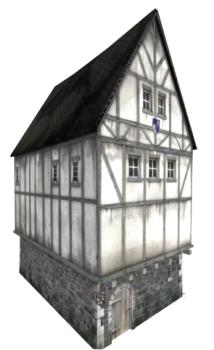
\includegraphics[scale=0.5]{figures/house_pers_350px.png}} & \raisebox{-\totalheight}{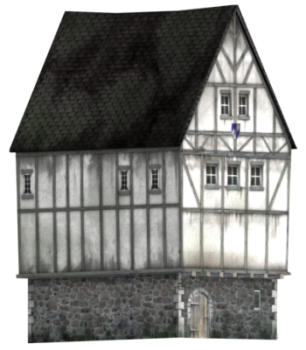
\includegraphics[scale=0.5]{figures/house_para_350px.png}} \\ 
	\hline 
\end{tabular}

\subsubsection{Lochkamera}

\begin{itemize}
	\item Eine Lochkamera besteht aus einem Kameragehäuse mit einem sehr kleinen Loch durch das das Licht eindringen kann
	\item Das Bild formt sich an der Rückseite des Kameragehäuses und steht auf dem Kopf \\
	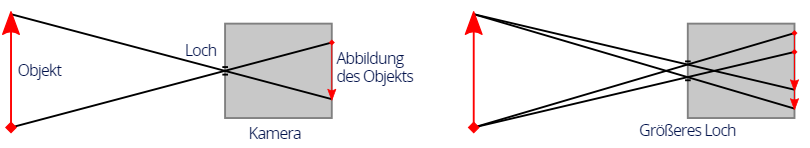
\includegraphics[scale=0.5]{figures/pinhole1.png}
	\item Ein größeres Loch hat den Vorteil, dass mehr Licht in die Kamera eindringen kann, was zu kürzeren Belichtungszeiten führt
	\item Der Nachteil ist, dass sich Projektion überlagern und das Bild unscharf wird
	\item In der Computergrafik wird meist ein idealisiertes Kameramodell mit einem unendlich kleinen Loch verwendet
	\item Dieses Kameramodel kann keine Tiefenunschärfe simulieren, d.h. alle Objekte werden scharf abgebildet
	\item Desweiteren wird angenommen, dass das Bild auf einer imaginären Bildebene vor dem Projektionszentrum erzeugt wird, sodass das Bild nicht mehr auf dem Kopf steht \\
	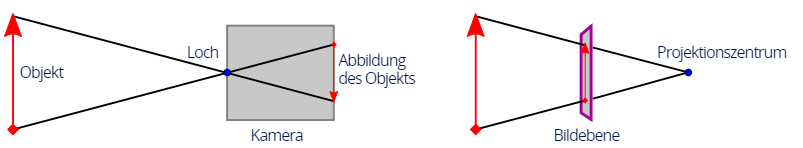
\includegraphics[scale=0.5]{figures/pinhole2.png}
\end{itemize}

\subsubsection{Perspektivische Projektion}

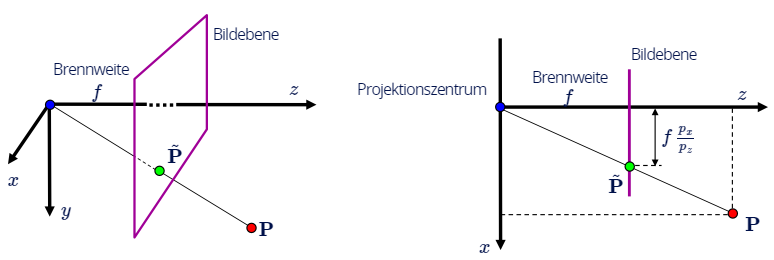
\includegraphics[scale=0.5]{figures/projection.png}

\begin{itemize}
	\item Die Projektionsvorschrift zur Abbildung eines 3D Punkts $P = (p_x, p_y, p_z)^\top$ auf einen Punkt $\widetilde{P} = (\widetilde{p}_x, \widetilde{p}_y, \widetilde{p}_z)^\top$ auf der Bildebene der Kamera lautet:
	\begin{equation}
		\widetilde{P} = (f \frac{p_x}{p_z}, f \frac{p_y}{p_z}, f)^\top
	\end{equation}
	\item Dies leitet sich sofort aus der Zeichnung mit Hilfe des Strahlensatzes ab, da
	\begin{equation}
		\frac{\widetilde{p}_x}{f} = \frac{p_x}{p_z} \text{ und }  \frac{\widetilde{p}_y}{f} = \frac{p_y}{p_z}
	\end{equation}
	\item Bei Verwendung von homogenen Koordinaten kann die perspektivische Projektion als lineare Abbildung mittels einer $4 \times 4$ Matrix geschrieben werden: \\
	\begin{equation}
		\begin{split}
			\widetilde{P} &= \begin{pmatrix}
			\widetilde{p}_x \\
			\widetilde{p}_y \\
			\widetilde{p}_z
			\end{pmatrix} = \begin{pmatrix}
			f \frac{p_x}{p_z} \\
			f \frac{p_y}{p_z} \\
			f
			\end{pmatrix} \in \mathbb{R}^3 \mapsto \underline{\widetilde{P}} = \begin{pmatrix}
			f p_x \\
			f p_y \\
			f p_z \\
			p_z
			\end{pmatrix} \in \mathbb{H}^3 \\
			\underline{\widetilde{P}} &= \begin{pmatrix}
			f p_x \\
			f p_y \\
			f p_z \\
			p_z
			\end{pmatrix} = \ \underbrace{\begin{bmatrix}
			f & 0 & 0 & 0 \\
			0 & f & 0 & 0 \\
			0 & 0 & f & 0 \\
			0 & 0 & 1 & 0
			\end{bmatrix}}_A \begin{pmatrix}
			p_x \\
			p_y \\
			p_z \\
			1
			\end{pmatrix} \\
			\underline{\widetilde{P}} &= A \underline{P}
		\end{split}
	\end{equation}
\end{itemize}

\subsubsection{Perspektivische Projektion in OpenGL}

\begin{itemize}
	\item  In OpenGL zeigt die Kamera in die negative $z$-Richtung, damit gilt: \\
	\begin{equation}
		\begin{split}
			\underline{\widetilde{P}} &= \begin{pmatrix}
			f p_x \\
			f p_y \\
			f p_z \\
			-p_z
			\end{pmatrix} = \underbrace{\begin{bmatrix}
			f & 0 & 0 & 0 \\
			0 & f & 0 & 0 \\
			0 & 0 & f & 0 \\
			0 & 0 & -1 & 0
			\end{bmatrix}}_A \begin{pmatrix}
			p_x \\
			p_y \\
			p_z \\
			1
			\end{pmatrix} \\
			\underline{\widetilde{P}} &= A \underline{P}
		\end{split}
	\end{equation} \\
	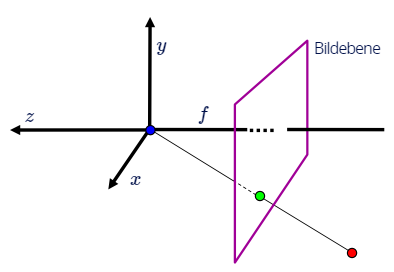
\includegraphics[scale=0.5]{figures/projection_negz.png}
	\item In OpenGL gibt es eine sogenannte NEar- und eine Far-Clipping-Ebene
	\item Die Near-Ebene und die Far-Ebene verlaufen parallel zur Bildebene
	\item Es sollen nur Punkte mit einer $z$-Koordinate dargestellt werden, die innerhalb des von der Near- und der Far-Ebene definierten Bereichs fallen
	\item Zu diesem Zweck soll eine neue lineare Abbildung definiert werden, bei der für die $z$-Koordinate der Punkte auf der Near-Ebene gelten soll: \\
	$p_z = -z_n \mapsto \widetilde{p}_z = -1$ \\
	und für Punkte auf der Far-Ebene: \\
	$p_z = -z_f \mapsto \widetilde{p}_z = 1$ \\
	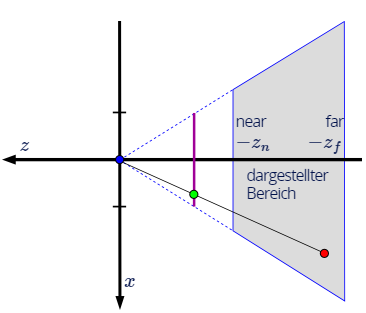
\includegraphics[scale=0.5]{figures/projection_clipping_map.png}
	\item Um dies zu erreichen, werden zwei neue Parameter $\alpha$ und $\beta$ in die lineare Transformationsmatrix hinzugefügt \\
	\begin{equation}
		\underline{\widetilde{P}} = \begin{pmatrix}
		f p_x \\
		f p_y \\
		\alpha p_z + \beta \\
		-p_z
		\end{pmatrix} = \begin{bmatrix}
		f & 0 & 0 & 0 \\
		0 & f & 0 & 0 \\
		0 & 0 & \alpha & \beta \\
		0 & 0 & -1 & 0
		\end{bmatrix} \begin{pmatrix}
		p_x \\
		p_y \\
		p_z \\
		1
		\end{pmatrix} \in \mathbb{H}^3
	\end{equation}
	\item Für den projizierten Punkt in kartesischen Koordinaten gilt damit: \\
	\begin{equation}
		\widetilde{P} = (\widetilde{p}_x, \widetilde{p}_y, \widetilde{p}_z)^\top = (f \frac{p_x}{-p_z}, f \frac{p_y}{-p_z}, - \alpha + \frac{\beta}{-p_z})^\top \in \mathbb{R}^3
		\end{equation}
		\item Nun können $\alpha$ und $\beta$ aus den Bedingungen für die Abbildung der $z$-Koordinate bestimmt werden: \\
		\begin{equation}
			\begin{split}
				p_z &= -z_n \mapsto \widetilde{p}_z = -1 \implies -\alpha + \frac{\beta}{z_n} = -1 \\
				p_z &= -z_f \mapsto \widetilde{p}_z = 1 \implies -\alpha + \frac{\beta}{z_f} = 1			\end{split}
	\end{equation}
	\item Auflösen des Gleichungssystems nach $\alpha$ und $\beta$ liefert: \\
	\begin{equation}
		\begin{split}
			\alpha &= \frac{z_f + z_n}{z_n - z_f} \\
			\beta &= \frac{2 z_f z_n}{z_n - z_f}
		\end{split}
	\end{equation}
	\item Damit gilt für die neue Projektionsamtrix: \\
	\begin{equation}
		\begin{split}
			\underline{\widetilde{P}} &= \underbrace{\begin{bmatrix}
			f & 0 & 0 & 0 \\
			0 & f & 0 & 0 \\
			0 & 0 & \frac{z_f + z_n}{z_n - z_f} & \frac{2 z_f z_n}{z_n - z_f} \\
			0 & 0 & -1 & 0
			\end{bmatrix}}_A \begin{pmatrix}
			p_x \\
			p_y \\
			p_z \\
			1
			\end{pmatrix} \\
			\underline{\widetilde{P}} &= A \underline{P}
		\end{split}
	\end{equation}
	\item Bisher haben wir zwar den Abstand der Bildebene zur Kamera druch die Brennweite $f$ definiert, jedoch keine Aussage über die Größe der Bildebene in $x$- und $y$-Richtung getroffen
	\item Letztendlich ist nur das Verhältnis zwischen der Größe der Bildebene und der Brennweite entscheidend, das über den Öffnugnswinkel $\Theta$ eindeutig definiert ist. Alle Konfigurationen mit dem gleichen Öffnungswinkel resultieren in dem gleichen Bild (nur mit skalierten $x$- und $y$-Koordinaten).
	\item In OpenGL wird die Größe der Bildebene daherimmer so gewählt, dass die resultierenden $x$- und $y$-Koordinaten im Bereich [-1;1] liegen.
	\item Für einen gegebenen Öffnungswinkel ergibt sich daher für die Brennweite (gemäß Zeichnung): \\
	\begin{equation}
	\frac{f}{1} = \frac{\cos (0.5 \Theta)}{\sin (0.5 \Theta)} \iff f = cotan (0.5 \Theta)
	\end{equation} \\
	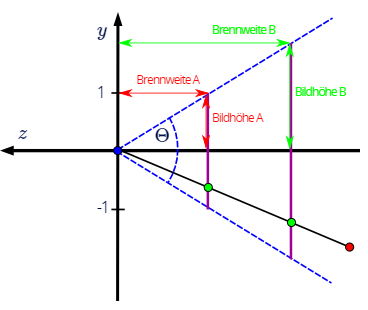
\includegraphics[scale=0.5]{figures/projection_ysize.png}
	\item Für die Projektion vom Kamerakoordinatensystem in die Bildebene ist die GL\_PROJECTION Matrix verantwortlich.
	\item Die Manipulation dieser Matrix wird aktiviert durch \\
	\begin{lstlisting}
glMatrixMode(GL_PROJECTION);
	\end{lstlisting}
	\item Alle Funktionen zur Matrixmanipulation, wie glLoadIdentity, glLoadMatrix, glMultMatrix, glRotate, glScale, glTranslate, glPushMatrix, glPopMatrix, gluPerspective werden dann auf der GL\_PROJECTION Matrix ausgeführt.
	\item Der aktuelle Zustand der GL\_PROJECTION Matrix beeinflusst die Transformationen der Objekte nur dann, wenn diese gezeichnet werden(OpenGL als Zustandsmaschine)
	\item Erzeugen einer perspektivischen Projektionsmatrix in OpenGL: \\
	\begin{lstlisting}
glMatrixMode(GL_PROJECTION);
glLoadIdentity();
gluPerspective(
	fovy,
	aspect,
	near,
	far
);
	\end{lstlisting}
	\begin{equation}
		\begin{split}
			A &= \begin{bmatrix}
			\frac{f}{aspect} & 0 & 0 & 0 \\
			ß & f & 0 & 0 \\
			0 & 0 & \frac{far + near}{near - far} & \frac{2 \times far \times near}{near - far} \\
			0 & 0& -1 & 0
			\end{bmatrix} \\
			\text{mit } f &= cotan(0.5 \times fovy) \\
			\text{und } aspect &= w/h
		\end{split}
	\end{equation} \\
	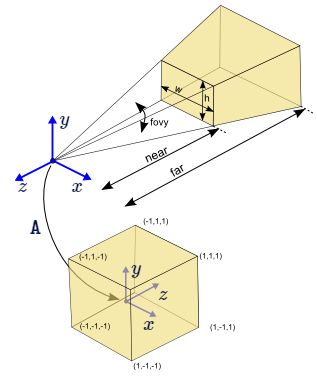
\includegraphics[scale=0.5]{figures/gluperspective.png}
\end{itemize}

\subsubsection{Dolly Zoom oder Vertigo Effekt}

\begin{itemize}
	\item Die Idee des ''Dolly Zoom''-Effekts ist, eine Translation der Kamera in $z$-Richtung (''Dolly'') durch eine entsprechende Veränderung der Brennweite (''Zoom'') auszugleichen
	\item Mathematisch ist die Möglichkeit einer Kompensation leicht aus der Projektionsgleichung zu entnehmen, da für die $y$-Koordinate eines projizierten Punkts gilt: \\
	\begin{equation}
		\widetilde{p}_y = f \frac{p_y}{-p_z}
	\end{equation}
	\item Da es nur eine Brennweite $f$ gibt, aber typischerweise viele 3D-Punkte mit unterschiedlichem Tiefenwert $p_z$ in einer 3D Szene, kann die Kompensation nur für einen bestimmten Tiefenwert gelingen. Es entsteht ein interessanter perspektivischer Effekt.
	\item[] 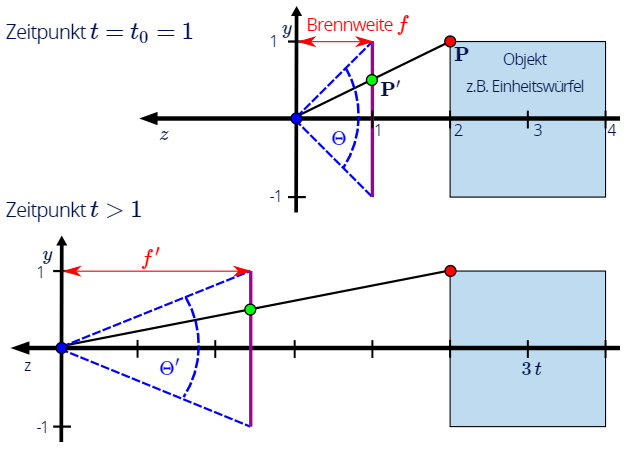
\includegraphics[scale=0.5]{figures/dolly_zoom.png}
\end{itemize}

\subsubsection{Transformation der Kamera}

\begin{itemize}
	\item Bisher wurde angenommen, dass sich das Projektionszentrum der Kamera im Urpsrung des globalen Weltkoordinatensystems befindet
	\item Wird eine Transformation $T_{cam}$ auf die Kamera angewendet, gilt für die Projektion eines Punkts \textbf{P} aus einem lokalen Objektkoordinatensystems:
	\begin{equation}
		\underline{\widetilde{P}} = AT_{cam}^{-1} T_{obj} \underline{P}
	\end{equation}
	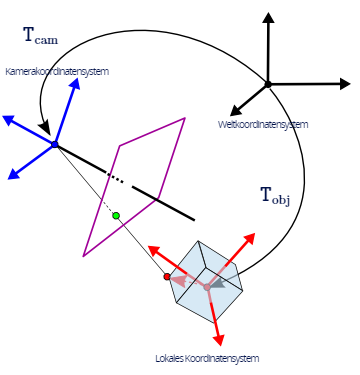
\includegraphics[scale=0.5]{figures/local2cam1.png}
	\item Abbildungsvorschrift für homogene Punkte:
	\begin{equation}
		\underline{\widetilde{P}} = AT_{cam}^{-1} T_{obj} \underline{P}
	\end{equation}
	Dabei beschreibt die $4 \times 4$ Matrix
	\begin{itemize}
		\item $T_{obj}$ die Transformation vom lokalen Koordinatensystem ins Weltkoordinatensystem
		\item $T_{cam}^{-1}$ die Transformation vom Weltkoordinatensystem ins Kamerakoordinatensystem
		\item $A$ die Transformation vom Kamerakoordinatensystem in die Bildebene
	\end{itemize}
	\item Die Transformationsmatrizen ergeben sich durch Betrachten der Basisvektoren der Koordinatensysteme (wie in den vorherigen Kapiteln besprochen)
	\item Die Transformationsmatrix $T_{obj}$ transformiert einen Punkt vom lokalen ins Weltkoordinatensystem
	\begin{equation}
		T_{obj} = \begin{bmatrix}
		\widetilde{b_x} & \widetilde{b}_y & \widetilde{b}_z & C_b \\
		0 & 0 & 0 & 1 
		\end{bmatrix}
	\end{equation}
	\item Die Transformationsmatrix $T_{cam}$ transformiert einen Punkt vom Kamera- ins Weltkoordinatensystem
	\begin{equation}
		\begin{split}
			T_{cam} &= \begin{bmatrix}
			\widetilde{a}_x & \widetilde{a}_y & \widetilde{a}_z & C_a \\
			0 & 0 & 0 & 1
			\end{bmatrix} \\
			&= \begin{bmatrix}
			R_a & C_a \\
			0^\top & 1
			\end{bmatrix}
		\end{split}
	\end{equation}
	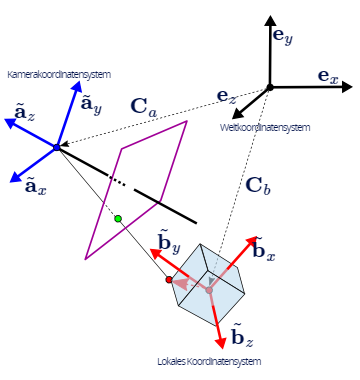
\includegraphics[scale=0.5]{figures/local2cam2.png}
	\item Für die inverse Tranformation $T_{cam}^{-1}$ vom Welt- ins Kamerakoordinatensystem, ergibt sich mit $R_a^{-1} = R_a^\top$:
	\begin{equation}
		T_{cam}^{-1} = \begin{bmatrix}
		R_a & C_a \\
		0^\top & 1
		\end{bmatrix}^{-1} = \begin{bmatrix}
		R_a^\top & -R_a^\top C_a \\
		0^\top & 1
		\end{bmatrix}
	\end{equation}
\end{itemize}

\subsubsection{Transformation der Kamera in OpenGL}

\begin{itemize}
	\item Abbildungsvorschrift für homogene Punkte:
	\begin{equation}
		\underline{\widetilde{P}} = A  \underbrace{T_{cam}^{-1} T_{obj}}_{T_{modelview}}  \underline{P}
	\end{equation}
	\begin{itemize}
		\item In OpenGL werden alle Transformationen außer der Projektionsmatrix $A$ zu einer sogenannten GL\_MODELVIEW Matrix zusammengefasst
		\item Die GL\_MODELVIEW Matrix beschreibt somit direkt die Transformation vom jeweiligen lokalen Koordinatensystem ins Kamerakoordinatensystem
		\item Die GL\_PROJECTION Matrix $A$ beschreibt die Abbildung vom Kamerakoordinatensystem in die Bildebene
	\end{itemize}
\end{itemize}

\subsubsection{gluLookAt}

\begin{itemize}
	\item Zur einfachen Definition der Matrix $T_{cam}^{-1}$ existiert die GLU-Funktion
	\begin{lstlisting}
gloLookAt(
	eyex,
	eyey,
	eyez,
	refx,
	refy,
	refz,
	upx,
	upy,
	upz
);
	\end{lstlisting}
	\item Durch Definition eines Aufpunkts $C_{eye}$, eines anvisierten Referenzpunkts $P_{ref}$ und eines Vektors $v_{up}$ (der definiert, in welche Richtung die $y$-Koordinate der Kamera zeigt) ergeben sich die Basisvektoren des Kamerakoordinatensystems zu:
	\begin{equation}
		\begin{split}
			d &= P_{ref} - c_{eye} \\
			\widetilde{a}_z &= \frac{d}{\mid d \mid} \\
			v' &= \frac{v_{up}}{\mid v_{up} \mid} \\
			\widetilde{a}_x &= v' \times \widetilde{a}_z \\
			\widetilde{a}_y &= \widetilde{a}_z \times \widetilde{a}_x \\
			R_a &= \begin{bmatrix}
			\widetilde{a}_x & \widetilde{a}_y & \widetilde{a}_z
			\end{bmatrix} \implies T_{cam}^{-1} = \begin{bmatrix}
			R_a^\top & -R_a^\top C_{eye} \\
			0^\top & 1
			\end{bmatrix}
		\end{split}
	\end{equation}
	\item Welche Transformationen durchlaufen die Punkte des kleineren Würfels? \\
	\begin{minipage}{.5\textwidth}
		\begin{lstlisting}
glMatrixMide(GL_PROJECTION);
glLoadIdentitiy();
gluPerspective(...);

glMatrixMode(GL_MODELVIEW);
glLoadIdentity();
gluLookAt(...);

glRotatef(...);
glTranslatef(...);
glScalef(...);
	\end{lstlisting}
	\end{minipage}
	\begin{minipage}{.5\textwidth}
		\ \\
		$T_{projection} ) I$ \\
		$T_{projection} ) I A$ \\
		\\
		\\
		$T_{modelview} = I$ \\
		$T_{modelview} = IT_{cam}^{-1}$ \\
		\\
		\\
		$T_{modelview} = IT_{cam}^{-1}T_r$ \\
		$T_{modelview} = IT_{cam}^{-1}T_r T_t$ \\
		$T_{modelview} = IT_{cam}^{-1}T_r T_t T_s$ \\
	\end{minipage}
	\begin{equation}
		\begin{split}
			\underline{\widetilde{P}} &= T_{projection} T_{modelview} \underline{P} \\
			&= AT_{cam}^{-1} T_r T_t T_s \underline{P}
		\end{split}
	\end{equation}
\end{itemize}

\subsubsection{Per-Vertex Operations}

Bei Verwendung der Fixed-Function-Pipeline werden folgende Transformationen auf die Vertex Daten angewendet

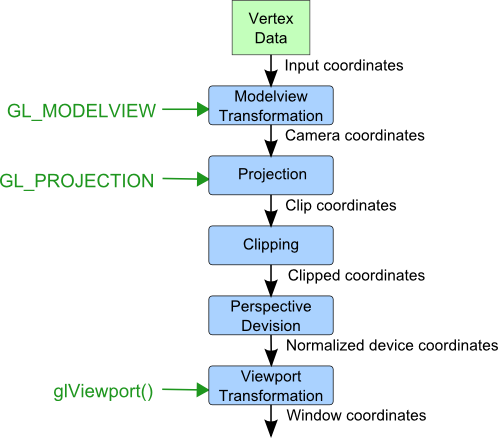
\includegraphics[scale=1]{figures/pervertex_fixedfunction_pipeline.png}

\subsubsection{Perspektivische Division}

\begin{itemize}
	\item Die so genannte ''perspektivische Division'' überführt die projizierten Punkte in homogenen Koordinaten ins kartesische Koordinatensystem durch Division mit der letzten Koordinate:
	\begin{equation}
		\underline{P} = \begin{pmatrix}
		p_x \\
		p_y \\
		p_y \\
		p_w
		\end{pmatrix} \in \mathbb{H}^3 \mapsto P = \begin{pmatrix}
		\frac{p_x}{p_w} \\
		\frac{p_x}{p_y} \\
		\frac{p_z}{p_w}
		\end{pmatrix} \in \mathbb{R}^3
	\end{equation}
\end{itemize}

\subsubsection{Clipping}

\begin{itemize}
	\item Die Projektionsmatrix wurde so konstruiert, dass nach Projektionen und der perspektivischen Division alle $x$, $y$ und $z$-Koordinaten innerhalb des sichtbaren Volumens auf den Bereich [-1;1] abgebildet werden
	\item Alle Primitiven, die vollständig außerhalb dieses Bereichs liegen, müssen nicht gezeichnet werden
	\item Durch Prüfen auf den Bereich [-1;1] wäre es leicht, das Clipping nach der perspektivischen Division durchzuführen
	\item In OpenGL wird das Clipping jedoch vor der perspektivischen Division durchgeführt. Warum?
	\item Anstatt auf den Bereich [-1;1] zu prüfen, kann genau so schnell auf den Bereich $[-p_w;p_w]$ geprüft werden
	\begin{equation}
		-p_w < p_x < p_w \mapsto -1 < \frac{p_x}{p_w} < 1
	\end{equation}
	\item Dies hat den Vorteil, dass
	\begin{itemize}
		\item für den Fall $p_w = 0$ keine besondere Behandlung, benötigt wird und
		\item die Division für die geclippten Koordinaten nicht mehr durchgeführt werden muss
	\end{itemize}
\end{itemize}

\subsubsection{Viewport Transformation}

\begin{itemize}
	\item Im letzten Transformationsschritt werden die Koordinaten im Bereich [-1;1] auf Bildschirmkoordinaten skaliert
	\item Dazu existiert in OpenGL der Befehl \\
	\begin{lstlisting}
glViewport(
	int ix,
	int iy,
	int width,
	int height
);
	\end{lstlisting}
	\item Dabei geben $ix$ und $iy$ die linke untere Ecke des Viewports und \textit{width} und \textit{height} die Größe an (jeweils in der Einheit Pixel) \\
	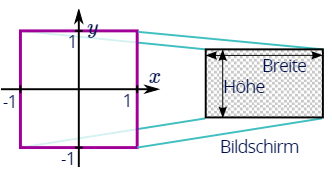
\includegraphics[scale=0.5]{figures/viewport_transformation.png}
\end{itemize}

\subsubsection{Fluchtpunkte}

\begin{itemize}
 \item Durch eine perspektivische Abbildung werden parallele Geraden im 3D Raum auf nicht parallele Geraden in der 2D Bildebene abgebildet
 \item Der 2D Schnittpunkt dieser Geraden in der Bildebene wird \textbf{Fluchtpunkt} genannt
 \item Jede Raumrichtung kann ihren eigenen (oder keinen) Fluchtpunkt besitzen
 \item Je nachdem, wie viele FLuchtpunkte existieren, wird die Projektion als 1-, 2-, oder 3-Punktperspektive bezeichnet \\
 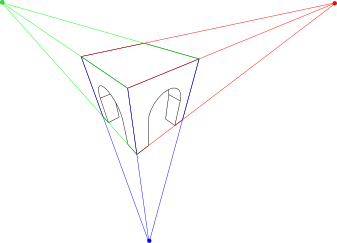
\includegraphics[scale=0.5]{figures/vanishing_points.png}
\end{itemize}

\subsection{Z-Buffer}

\subsubsection{Tiefentest}

\begin{itemize}
	\item In den vorherigen Beispielen wurden \textit{glEnable(GL\_DEPTH\_TEST)} und \\
	\textit{GlClear(GL\_DEPTH\_BUFFER\_BIT)} verwendet, ohne dass deren Funktion diskutiert wurde.
	\item Der Aufruf \textit{glEnable(GL\_DEPTH\_TEST)} dient dazu, den Tiefentest in OpenGL zu aktivieren
	\item Bei deaktiviertem Tiefentest werden die Primitiven in der Reihenfolge in den Framebuffer geschrieben, in der sie die OpenGL-Pipeline durchlaufen.
	\item Das heißt, später gezeichnete Primitive werden früher gezeichnete überdecken
	\item Das ist typischerweise nicht das gewünschte Verhalten.
	\item Stattdessen sollen Primitive, die aus Sicht der Kamera näher liegen weiter entfernte verdecken und zwar unabhängig von der Reihenfolge des Zeichnens.
	\item Idealerweise sollte die Entscheidung pro gezeichnetem Pixel im Framebuffer erfolgen, da sich die einzelnen Primitve durchdringen können.
	\item In OpenGL wird als Tiefentest das Z-Buffer-Verfahren verwendent. \\
	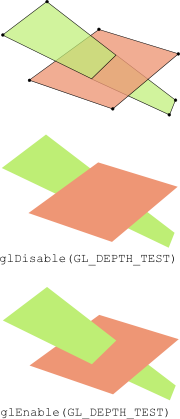
\includegraphics[scale=1]{figures/depthtest_example.png}
\end{itemize}

\subsubsection{Z-Buffer-Verfahren}

\begin{itemize}
	\item Obwohl eigentlich die $z$-Koordinate im Kamerakoordinatensystem entscheidend ist, kann der Tiefentest auch noch nach der perspektivischen Division durchgeführt werden, da die Tiefenrelation erhalten bleiben.
	\item Wenn ''Normalized device coordinates'' verwendet werden, dreht sich allerdings bezüglich des Kamerakoordinatensystems die $z$-Achse um, d.h. weiter entfernte Punkte haben ein größeres $z$ (speziell ist dabei das ausnahmsweise linkshändige Koordinatensytem).
	\item Für Punkte, die im Kamerakoordinatensystem auf der Near-Ebene lagen, gilt nun $\widetilde{p}_z = -1$ bzw. auf der Far-Ebene gilt $\widetilde{p}_z = 1$. \\
	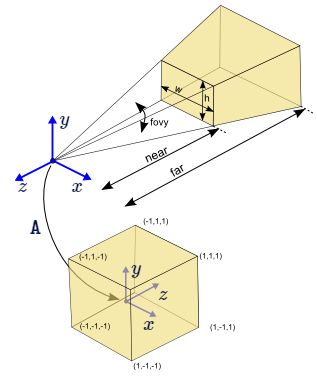
\includegraphics[scale=0.5]{figures/gluperspective.png}
	\item Das Z-Buffer-Verfahren benötigt, neben dem normalen Framebuffer, derdie Farbinformation aufnimmt, einen Depth-Buffer der gleichen Größe, der die Tiefenwerte aufnimmt. \\
	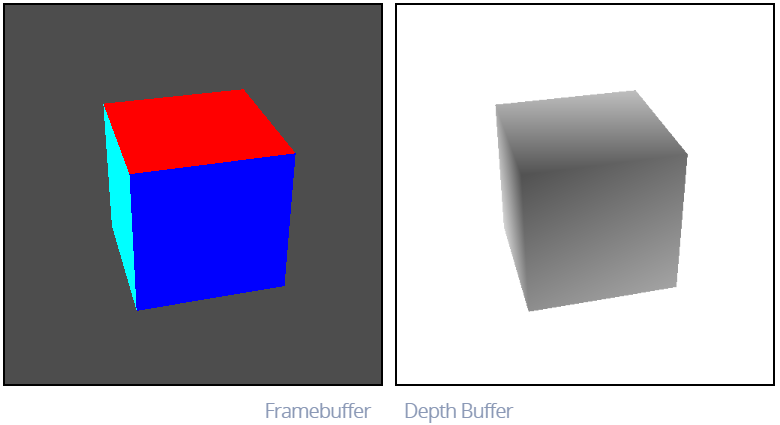
\includegraphics[scale=0.5]{figures/frame_vs_depthbuffer.png}
	\item Zu Beginn des Rendervorgangs wird der Depth-Buffer mit dem $z$-Wert der Far-Ebene initialisiert. Dazu dient in OpenGL der Befehl \textit{glClear(GL\_DEPTH\_BUFFER\_BIT)}.
	\item Das Schreiben eines Pixels in den Frame- und Depth-Buffer geschieht während der Per-Fragment-Operationen in der OpenGL-Pipeline.
	\item Der Tiefenwert für jedes Pixel wird vom Rasterisierer aus den transformierten Vertex-Daten interpoliert.
	\item Ist der Tiefenwert für das Pixel kleiner als der aktuell im Depth-Buffer gespeicherte, wird der Farbwert in den Framebuffer und der Tiefenwert in den Depth-Buffer geschrieben, ansonsten bleiben beide unverändert. \\
	\begin{lstlisting}
FOR each primitiv
	FOR each pixel of primitive at position (x,y) with colour c and depth d
		IF d < depthbuffer(x,y)
			framebuffer(x,y) = c
			depthbuffer(x,y) = d
		END IF
	END FOR
END FOR
	\end{lstlisting}
\end{itemize}

\subsubsection{Z-Fighting}

\begin{itemize}
	\item Der Depth-Buffer hat nur eine bestimmte Genauigkeit. Typischerweise ganzzahlige Werte mit 16, 24 oder 32 Bit Genauigkeit.
	\item Das Interval [-1.0;1.0] wird auf [0.0;1.0] abgebildet und dann auf [0;MAX\_INT], z.B. [0;65535] bei 16 Bit
	\item Dabei wird auf den nächsten ganzzahligen Wert gerundet.
	\item Da bei den ''Normalized device coordinates'' bereits durch $p_w$ geteilt wurde, sind die Rundungsfehler für Objekte nah an der Kamera damit kleiner (und deren Tiefengenauigkeit damit größer).
	\item Daher kommt es bei weit entfernten Primitiven, die dort nah beieinander liegen, gelegentlich zum so genannenten ''Z-Fighting'', da durch die Ungenauigkeiten in den $z$-Werten zufällig mal das eine, mal das andere, einen kleineren $z$-Wert hat und dargestellt wird.
	\item Um Z\_Fighting zu beheben, ist es wichtig, die Near- und Far-Ebene möglichst geschickt zu wählen, da diese letztendlich den $z$-Bereich definieren, auf die sich die möglichen ganzzahligen Tiefenwerte verteilen.
	\item Daher sollte die Near- und Far-Ebene möglichst dicht beieinander gewählt werden, so dass diese die darzustellende 3D-Szene gerade noch komplett umschließen. \\
	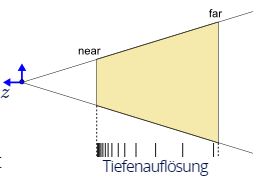
\includegraphics[scale=0.5]{figures/depthbuffer_resolution.png}
\end{itemize}

\subsection{Parallelprojektion}

\subsubsection{Parallelprojektion}

\begin{itemize}
	\item Bei der Parallelprojektion werden die Objekte mit größerem Abstand zum Betrachter bzw. Kamera nicht kleiner
	\item Es existieren keine Fluchtpunkte
\end{itemize}

\begin{tabular}{|c|c|}
	\hline Perspektivische Projektion & Parallelprojektion \\ 
	\hline \raisebox{-\totalheight}{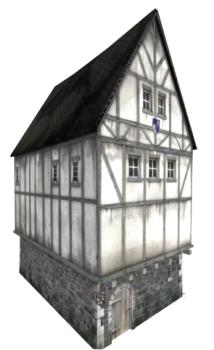
\includegraphics[scale=0.5]{figures/house_pers_350px.png}} & \raisebox{-\totalheight}{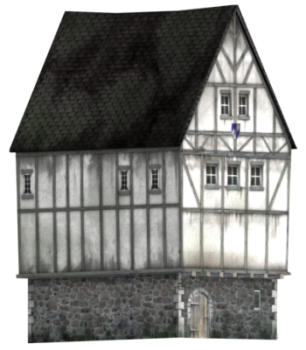
\includegraphics[scale=0.5]{figures/house_para_350px.png}} \\ 
	\hline 
\end{tabular}

\begin{itemize}
	\item Die Projektionsstrahlen verlaufen parallel, d.h. das Projektionszentrum liegt im Unendlichen
	\item Die Projektionsvorschrift zur Abbildung eines 3D Punkts $P = (p_x, p_y, p_z)^\top$ auf einen Punkt $\widetilde{P} = (\widetilde{p}_x, \widetilde{p}_y, \widetilde{p}_z)^\top$ auf der Bildebene der Kamera lautet: \\
	\begin{equation}
		\widetilde{P} = (p_x, p_y, 0)^\top
	\end{equation}
	\item Bei Verwendung von homogenen Koordinaten kann die Parallelprojektion wieder als $4 \times 4$ Matrix geschrieben werden: \\
	\begin{equation}
		\begin{split}
			\underline{\widetilde{P}} &= \begin{pmatrix}
			p_x \\
			p_y \\
			0 \\
			1
			\end{pmatrix} = \underbrace{\begin{bmatrix}
			1 & 0 & 0 & 0 \\
			0 & 1 & 0 & 0 \\
			0 & 0 & 0 & 0 \\
			0 & 0 & 0 & 1
			\end{bmatrix}}_A \begin{pmatrix}
			p_x \\
			p_y \\
			p_z \\
			1
			\end{pmatrix} \\
			\underline{\widetilde{P}} &= A \underline{P}
		\end{split}
	\end{equation}
\end{itemize}

\subsubsection{Parallelprojektion in OpenGL}

\begin{itemize}
	\item Die $x$-, $y$- und $z$-Koordinaten des Sichtvolumens sollen sich wieder jeweils in den Bereich [-1;1] abbilden
	\item Um dies zu erreichen, werden pro Koordinate zwei neue Parameter $\alpha$ und $\beta$ in die lineare Transformationsmatrix hinzugefügt \\
	\begin{equation}
		A = \begin{bmatrix}
		\alpha & 0 & 0 & \beta_x \\
		0 & \alpha & 0 & \beta_y \\
		0 & 0 & -\alpha_z & \beta_z \\
		0 & 0 & 0 & 1
		\end{bmatrix}
	\end{equation}
	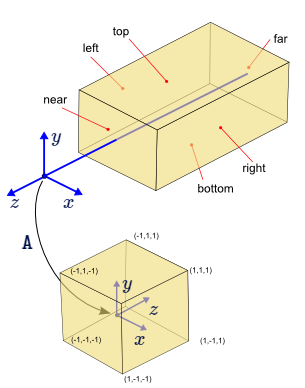
\includegraphics[scale=0.5]{figures/glortho.png}
	\item Beispielsweise soll für die $z$-Koordinate der Punkte auf der Near-Ebene gelten:
	\begin{equation}
			p_z = -z_n \mapsto \widetilde{p}_z = -1
	\end{equation}
	und für Punkte auf der Far-Ebene:
	\begin{equation}
		\begin{split}
			p_z &= -z_f \mapsto \widetilde{p}_z = 1 \\
			\underline{\widetilde{P}} &= \begin{pmatrix}
			\alpha_x p_x + \beta_x \\
			\alpha_y p_y + \beta_y \\
			-\alpha_z p_z + \beta_z \\
			1
			\end{pmatrix} = \begin{bmatrix}
			\alpha_x & 0 & 0 & \beta_x \\
			0 & \alpha_y & 0 & \beta_y \\
			0 & 0 & -\alpha_z & \beta_z \\
			0 & 0 & 0 & 1
			\end{bmatrix} \begin{pmatrix}
			p_x \\
			p_y \\
			p_z \\
			1
			\end{pmatrix} \in \mathbb{H}^3
		\end{split}
	\end{equation}
	\item Nun können $\alpha_z$ und $\beta_z$ aus den Bedingungen für die Abbildung der $z$-Koordinate bestimmt werden:
	\begin{equation}
		\begin{split}
			p_z &= -z_n \mapsto \widetilde{p}_z = -1 \implies \alpha_z z_n + \beta_z = -1 \\
			p_z &= -z_f \mapsto \widetilde{p}_z = 1 \implies \alpha_z z_f + \beta_z = 1
		\end{split}
	\end{equation}
	\item Auflösen des Gleichungssystems nach $\alpha_z$ und $\beta_z$ liefert:
	\begin{equation}
		\begin{split}
			\alpha &= \frac{2}{z_f - z_n} \\
			\beta_z &= -\frac{z_f + z_n}{z_f - z_n}
		\end{split}
	\end{equation}
	\item Nach analogen Rechnungen für die $x$- und $y$-Koordinate, ergibt sich die Projektionsmatrix zu:
	\begin{equation}
		A = \begin{bmatrix}
		\frac{2}{x_r - x_l} & 0 & 0 & -\frac{x_r + x_l}{x_r - x_l} \\
		0 & \frac{2}{y_t - y_b} & 0 & -\frac{y_t + y_b}{y_t - y_b} \\
		0 & 0 & \frac{-2}{z_f - z_n} & -\frac{z_f + z_n}{z_f - z_n} \\
		0 & 0 & 0 & 1
		\end{bmatrix}
	\end{equation}
	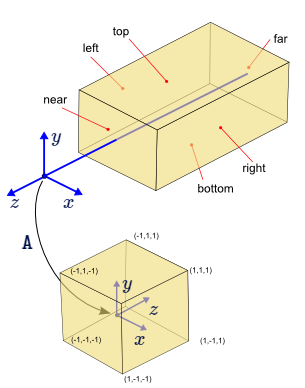
\includegraphics[scale=0.5]{figures/glortho.png}
	\item Erzeugen einer $4 \times 4$ Parallelprojektionsmatrix in OpenGL:
	\begin{lstlisting}
glMatrixMode(GL_PROJECTION);
glLoadIdentity();
glOrtho(left, right, bottom, top, near, far);
	\end{lstlisting}
	\begin{equation}
		A = \begin{bmatrix}
		\frac{2}{right - left} & 0 & 0 & -\frac{right + left}{right - left} \\
		0 & \frac{2}{^top - bottom} & 0 & -\frac{top + bottom}{top - bottom} \\
		0 & 0 & \frac{-2}{far - near} & -\frac{far + near}{far - near} \\
		0 & 0 & 0 & 1
		\end{bmatrix}
	\end{equation}
\end{itemize}

\subsubsection{Klassifikation planarer Projektionen}

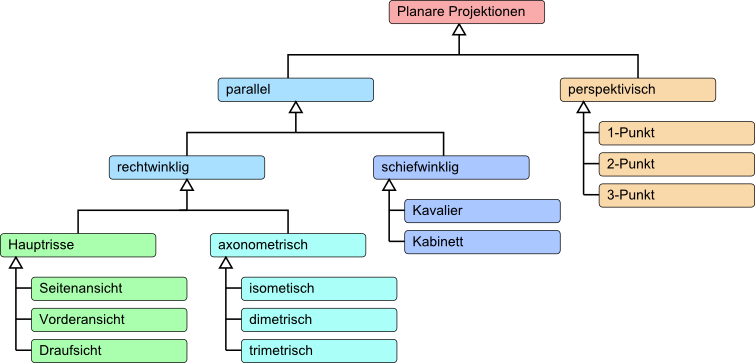
\includegraphics[scale=1]{figures/projection_classification.png}

\subsubsection{Rechtwinklige Projektion - Hauptrisse}

\begin{itemize}
	\item Hauptrisse sind Parallelprojektionen entlang der 3 Hauptrichtungen des kartesischen Koordinatensystems
	\item Insgesamt gibt es 6 Hauptrisse entlang $x, (-x), y, (-y), z$ und $(-z)$-Achse (Seitenansicht, Aufsicht, Vorderansicht)
	\item Hauptrisse sind beliebt bei Konstruktionszeichnungen (z.B. im Maschinenbau oder in der Architektur)
	\item Die verschiedenen Hauptrisse können z.B. durch eine zusätzliche 90 (oder 180) Grad Rotation erreicht werden
	\begin{equation}
		AT_{cam}^{-1} = AT_R(90^\circ)
	\end{equation}
	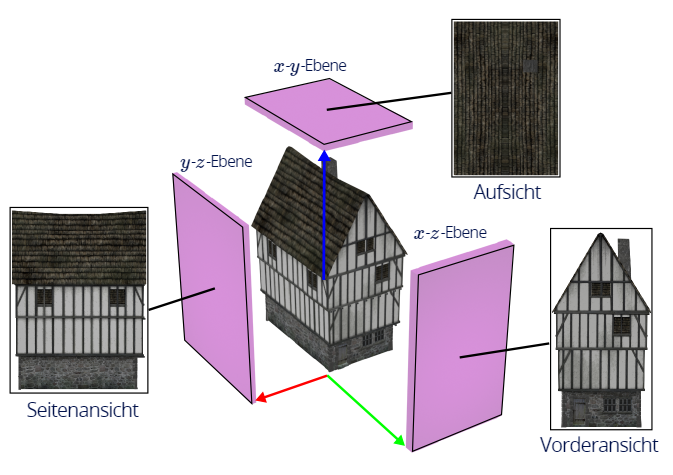
\includegraphics[scale=0.5]{figures/house_ortho.png}
\end{itemize}

\subsubsection{Rechtwinklige Projektion - Axonometrie}

\begin{itemize}
	\item Im Allgemeinen kann eine Rotation um die Achse $n$ mit dem Winkel $\alpha$ betrachtet werden
	\begin{equation}
		AT_{cam}^{-1} = AT_r (n, \alpha)
	\end{equation}
	\item Die resultierende Abbildung wird \textbf{rechtwinklige Projektion} genannt
	\item Die Klassifizierung der Projektion ergibt sich aus den Längen der abgebildeten Basisvektoren des kartesischen Koordinatensystems
	\begin{itemize}
		\item 3 Achsen die gleiche Länge: isometrisch
		\item 2 Achsen haben die gleiche Länge: dimetrisch
		\item Alle Achsen haben unterschiedliche Längen: trimetrisch
	\end{itemize}
	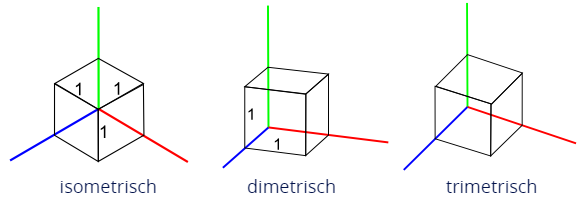
\includegraphics[scale=0.5]{figures/axonometic.png}
	\item Beispielsweise kann die Rotation um die $y$-Achse mit dem Winkel $\alpha$ und um die $x$-Achse mit $\beta$ betrachtet werden \\
	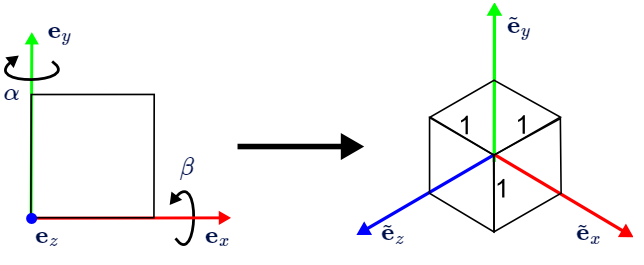
\includegraphics[scale=0.5]{figures/axonometic_ab.png}
	\begin{equation}
		\begin{split}
			AT_{cam}^{-1} &= AT_{r_x} (\beta) T_{r_y} (\alpha) \\
			&= \begin{bmatrix}
			1 & 0 & 0 & 0 \\
			0 & 1 & 0 & 0 \\
			0 & 0 & 0 & 0 \\
			0 & 0 & 0 & 1
			\end{bmatrix} \begin{bmatrix}
			1 & 0 & 0 & 0 \\
			0 & \cos \beta & -\sin \beta & 0 \\
			0 & \sin \beta & \cos \beta & 0 \\
			0 & 0 & 0 & 1
			\end{bmatrix} \begin{bmatrix}
			\cos \alpha & 0 & \sin \alpha & 0 \\
			0 & 1 & 0 & 0 \\
			-\sin \alpha & 0 & \cos \alpha & 0 \\
			0 & 0 & 0 & 1
			\end{bmatrix} \\
			&= \begin{bmatrix}
			1 & 0 & 0 & 0 \\
			0 & 1 & 0 & 0 \\
			0 & 0 & 0 & 0 \\
			\end{bmatrix} \begin{bmatrix}
			\cos \alpha & 0 & \sin \alpha & 0 \\
			\sin \beta \sin \alpha & \cos \beta & -\sin \beta \cos \alpha & 0 \\
			-\cos \beta \sin \alpha & \sin \beta & \cos \beta \cos \alpha & 0 \\
			0 & 0 & 0 & 1
			\end{bmatrix} \\
			&= \begin{bmatrix}
			\cos \alpha & 0 & \sin \alpha & 0 \\
			\sin \beta \sin \alpha & \cos \beta & -\sin \beta \cos \alpha & 0 \\
			0 & 0 & 0 & 0 \\
			0 & 0 & 0 & 1
			\end{bmatrix}
		\end{split}
	\end{equation}
	\item Die Basisvektoren bilden sich damit wie folgt ab:
	\begin{equation}
		\underline{\widetilde{e}}_x = \begin{pmatrix}
		\cos \alpha \\
		\sin \beta \sin \alpha \\
		0 \\
		1
		\end{pmatrix}, \underline{\widetilde{e}}_y = \begin{pmatrix}
		0 \\
		\cos \beta \\
		0 \\
		1
		\end{pmatrix}, \underline{\widetilde{e}}_z = \begin{pmatrix}
		\sin \alpha \\
		-\sin \beta \cos \alpha \\
		0 \\
		1
		\end{pmatrix}
	\end{equation}
	\item Somit können die Längen der abgebildeten Basisvektoren berechnet und die rechtwinklige Projektion in isometrisch, dimetrisch oder trimetrisch klassifiziert werden:
	\begin{equation}
		\begin{split}
			\mid \widetilde{e}_x \mid &= \sqrt{\cos^2 \alpha + (\sin \beta \sin \alpha)^2} \\
			\mid \widetilde{e}_y \mid &= \sqrt{\cos^2 \beta} \\
			\mid \widetilde{e}_z \mid &= \sqrt{\sin^2 \alpha + (\sin \beta \cos \alpha)^2}
		\end{split}
	\end{equation}
\end{itemize}

\subsubsection{Schiefwinklige Projektion}

\begin{itemize}
	\item Bei den schiefwinkligen Projektionen wird eine zusätzliche Scherung erlaubt
	\item Bei klassischen schiefwinkligen Projektionen werden meist zwei Koordinatenachsen durch die Abbildung nicht verändert und eine Scherung auf die Dritte angewendet
	\item Die Projektionsrichtung dieser dritten Achse kann mit zwei Winkeln $\alpha$ und $\beta$ angegeben werden (siehe Zeichnung)
	\item Der Winkel $\alpha$ bleibt bei der Projektion erhalten und entspricht dem Winkel zwischen der projizierten $z$- und $x$-Achse. Der Winkel $\beta$ steuert den Maßstab:
	\begin{itemize}
		\item Kavalierprojektion: $x : z = 1:1$
		\item Kabinettprojektion: $x : z = 2 : 1$
	\end{itemize}
	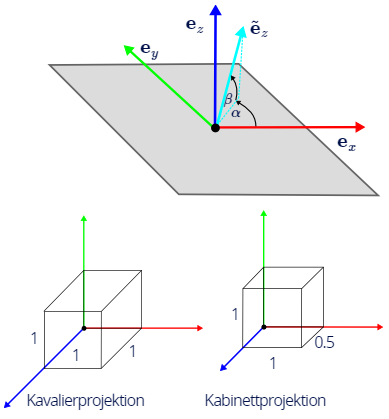
\includegraphics[scale=0.5]{figures/oblique.png}
	\item Allgemeine schiefwinklige Projektion:
	\begin{equation}
		AT_{cam}^{-1} = \begin{bmatrix}
		1 & 0 & 0 & 0 \\
		0 & 1 & 0 & 0 \\
		0 & 0 & 0 & 0 \\
		0 & 0 & 0 & 1
		\end{bmatrix} \begin{bmatrix}
		1 & 0 & \frac{-\cos \alpha}{\tan \beta} & 0 \\
		0 & 1 & \frac{\sin \alpha}{\tan \beta} & 0 \\
		0 & 0 & \frac{-1}{\sin \beta} & 0 \\
		0 & 0 & 0 & 1
		\end{bmatrix} = \begin{bmatrix}
		1 & 0 & \frac{-\cos \alpha}{\tan \beta} & 0 \\
		0 & 1 & \frac{\sin \alpha}{\tan \beta} & 0 \\
		0 & 0 & 0 & 0 \\
		0 & 0 & 0 & 1
		\end{bmatrix}
	\end{equation}
	\item Bei Kavalierprojektion: $\beta$ = 45 Grad
	\begin{equation}
		AT_{cam}^{-1} = \begin{bmatrix}
		1 & 0 & -\cos \alpha & 0 \\
		0 & 1 & \sin \alpha & 0 \\
		0 & 0 & 0 & 0 \\
		0 & 0 & 0 & 1
		\end{bmatrix}
	\end{equation}
	\item Bei Kabinettprojektion: $\beta$ = 63,4 Grad
	\begin{equation}
		AT_{cam}^{-1} = \begin{bmatrix}
		1 & 0 & \frac{-\cos \alpha}{2} & 0 \\
		0 & 1 & \frac{\sin \alpha}{2} & 0 \\
		0 & 0 & 0 & 0 \\
		0 & 0 & 0 & 1
		\end{bmatrix}
	\end{equation}
\end{itemize}

\section{Texturen}

\subsection{2D-Texturen}

\subsection{Texture-Mapping}

\begin{itemize}
	\item 2D-Texturen sind in der Regel quadratisch und mit den Parametern $s$ und $t$ im Bereich [0;1] parametisiert
	\item Zum Anwenden einer Textur ist es notwendig, die Abbildungsfunktion (''Texture-Mapping'') vom 2D-Raum auf eine 3D-Oberfläche zu definieren
	\item Diese wird typischerweise durch Zuweisen von Texturkoordinaten $(s,t)^\top$ zu 3D-Stützpunkten $P = (x,y,z)^\top$ des 3D-Modells erreicht
	\begin{equation}
		(s,t)^\top \mapsto (x,y,z)^\top
	\end{equation}
\end{itemize}

\subsubsection{Texturen in der OpenGL-Pipeline}

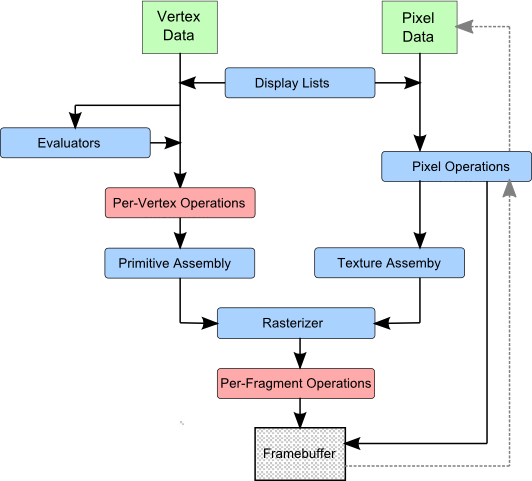
\includegraphics[scale=1]{figures/openglpipeline.png}

\begin{itemize}
	\item In OpenGL erfolgt das Setzen einer Texturkoordinate mit dem Befehl \textit{glTexCoord2f}
	\item Jeweils diejenige Texturkoordinate, die beim Zeichnen eines Stützpunkts gesetzt ist, wird dem Stützpunkt zugeordnet (OpenGL als Zustandsmaschine):
	\begin{lstlisting}
...
glBegin(GL_POLYGON);
glTexCoord2f(0.25f, 0.50f);
glVertex3f(-1.0f, 1.0f, 1.0f);
glTexCoord2f(0.25f, 0.25f);
glVertex3f(-1.0f, -1.0f, 1.0f);
glTexCoord2f(0.50f, 0.25f);
glVertex3f(1.0f, -1.0f, 1.0f);
glTexCoord2f(0.50f, 0.50f);
glVertex3f(1.0f, 1.0f, 1.0f);
glEnd();
...
	\end{lstlisting}
	\item Die Texturkoordinaten sind Teil der Vertx-Daten in der OpenGL-Pipeline und durchlaufen den linken Pfad der Pipeline
	\item Die Textur selbst besteht aus Pixel-Daten, die den rechten Pfad der Pipeline durchlaufen
	\item Die Texturpixel werden häufig als ''Texel'' bezeichnet
	\item Im Rasterisierer müssen für jedes ausgegebene Fragment (Pixel des Framebuffers) interpolierte Texturkoordinaten $(s,t)^\top$ berechnet werden
	\item Im Idealfall wird bei der Interpolation die Verzerrung durch die perspektivische Abbildung berücksichtigt (Perspective Texture-Mapping)
\end{itemize}

\subsubsection{Erstellen von 2D-Texturen in OpenGL}

\begin{itemize}
	\item Das Erstellen einer Textur geschieht in der Regel vor dem eigentlichen Rendern, also z.B. in der Funktion \textit{init()}
	\begin{itemize}
		\item Eine 2D-Textur kann erzeugt werden mit
		\begin{lstlisting}
glBindTexture(GL_TEXTURE_2D, texID);
glTexImage2D(
	GL_TEXTURE_2D,
	texLevel,
	texFormat,
	inWidth,
	inHeight,
	inBorder,
	inFormat,
	inType,
	inData
);
		\end{lstlisting}
		\item Dabei ist \textit{texID} ein Integer-Wert, der als eindeutiger Kennzeichner (''ID'') für die erzeugte Textur dient. Mit Hilfe der Funktion \textit{glGenTextures(1, \&texID)} kann ein solcher eindeutiger Kennzeichner generiert werden
		\item Beim Erstellen werden häufig auch weitere Parameter gesetzt, die die Darstellung der Textur beeinflussen
	\end{itemize}
\end{itemize}

\subsubsection{Aktivieren von 2D-Texturen in OpenGL}

\begin{itemize}
	\item Während des Render-Vorgangs muss zunächst die Textureinheit aktiviert werden:
	\begin{lstlisting}
glEnable(GL_TEXTURE_2D);
	\end{lstlisting}
	\item Zum Rendern mit einer bestimmten Textur wird deren eindeutige ID verwendet:
	\begin{lstlisting}
glBindTexture(GL_TEXTURE_2D, texID);
	\end{lstlisting}
	Dieser Befehl ''bindet'' die Textur mit der angegebenen ID an das Ziel \textit{GL\_TEXTURE\_2D}
	\item D.h. \textit{glBindTexture} hat mehrere Funktionen: Beim erstmaligen Aufruf mit einer neuen ID wird eine neue Textur erzeugt und ansonsten eine existierende Textur aktiviert
\end{itemize}

\subsubsection{Beispiel: Texturieren eines Würfels}

\begin{itemize}
	\item In diesem Beispiel soll ein Würfel texturiert werden
	\item Dazu müssen die entsprechenden Texturkoordinaten und Stützpunkte einander zugeordnet werden (in der Zeichnung sind diese mit den gleichen Farben kodiert) \\
	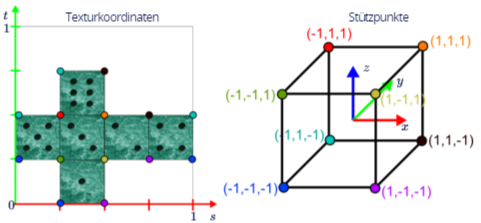
\includegraphics[scale=0.5]{figures/texture_dice.png}
\end{itemize}

\subsubsection{Wrap-Parameter}

\begin{itemize}
	\item Der \textit{GL\_TEXTURE\_WRAP}-Parameter bestimmt, wie sich das Texture-Mapping verhalten soll, wenn die Texturkoordinate $s$ oder $t$ den Zahlenbereich [0;1] verlässt
	\begin{lstlisting}
glTexParameter(
	GL_TEXTURE_2D,
	GL_TEXTURE_WRAP_S,
	GL_REPEAT
);
glTexParameter(
	GL_TEXTURE_2D,
	GL_TEXTURE_WRAP_T,
	GL_REPEAT
);
	\end{lstlisting}
	\item Mögliche Parameterwerte sind: \textit{GL\_CLAMP, GL\_REPEAT, GL\_CLAMP\_TO\_BORDER, GL\_CLAMP\_TO\_EDGE} oder \textit{GL\_MIRRORED\_REPEAT}
\end{itemize}

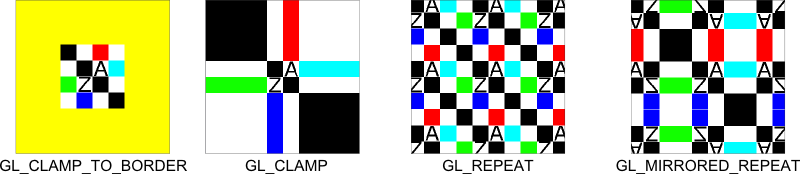
\includegraphics[scale=0.35]{figures/texture_wrap.png}

\subsubsection{Filter-Parameter}

\begin{itemize}
	\item Bei der Darstellung von Texturen müssen häufig Farbwerte für Texturkoordinaten berechnet werden, die nicht auf dem Pixelraster der zugrunde liegenden Rastergrafik liegen
	\item Ein Filter-Parameter erlaubt die Filtermethode festzulegen, mit welcher die Farbwerte in diesem Fall bestimmt werden soll
	\item \textit{GL\_TEXTURE\_MIN\_FILTER} setzt den Filter bei Verkleinerungen und \\
	\textit{GL\_TEXTURE\_MAG\_FILTER} für Vergrößerungen:
	\begin{lstlisting}
glTexParameter(
	GL_TEXTURE_2D,
	GL_TEXTURE_MAG_FILTER,
	GL_LINEAR
);
glTexParameter(
	GL_TEXTURE_2D,
	GL_TEXTURE_MIN_FILTER,
	GL_LINEAR
);
	\end{lstlisting}
	\item Mögliche Parameterwerte sind: \textit{GL\_NEAREST} oder \textit{GL\_LINEAR}
	\item Bei \textit{GL\_NEAREST} wird der Farbwert des Pixels verwendet, das den kleinsten Abstand zur Texturkoordinate hat (Nearest-Neighbor)
	\item Diese Operation ist sehr schnell, da die Texturkoordinaten lediglich auf einen ganzzahligen Pixel-Wert gerundet werden müssen und der zugehörige Farbwert $f$ dann direkt abgelesen werden kann
	\begin{equation}
		\begin{split}
			x_{nearest} &= int(s \times width + 0.5) \\
			y_{nearest} &= int(t \times height + 0.5) \\
			f_{nearest} &= f(x_{nearest}, y_{nearest})
		\end{split}
	\end{equation}
	\item Bei \textit{GL\_LINEAR} wird der Farbwert bilinear interpoliert
\end{itemize}

\subsubsection{Bilineare Interpolation}

\begin{itemize}
	\item Bei der bilinearen Interpolation an der Stelle $p = (x,y)^\top$ wird der Farbwert aus den 4 benachbarten Pixelwerten ermittelt, die exakt auf dem Pixelraster liegen. Diese seien gegeben als: $(x_1, y_1)^\top, (x_1, y_2)^\top, (x_2, y_1)^\top, (x_2, y_2)^\top$
	\item Zunächst werden per linearer Interpolation in $x$-Richtung die Farbwerte an den Hilfspositionen $q_1$ und $q_2$ bestimmt:
	\begin{equation}
		\begin{split}
			f(q_1) &= \frac{x_2 - x}{x_2 - x_1} f(x_1,y_1) + \frac{x - x_1}{x_2 - x_1} f(x_2, y_1) \\
			f(q_2) &= \frac{x_2 - x}{x_2 - x_1} f(x_1, y_2) + \frac{x - x_1}{x_2 - x_1} f(x_2, y_2)
		\end{split}
	\end{equation}
	\item Eine weitere lineare Interpolation, nun in $y$-Richtung, ergibt den Farbwert bei $p$:
	\begin{equation}
		f(p) = \frac{y_2 - y}{y_2 - y_1} f(q_1) + \frac{y - y_1}{y_2 - y_1} f(q_2)
	\end{equation}
	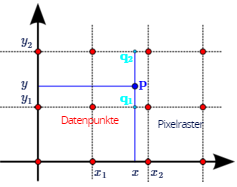
\includegraphics[scale=1]{figures/bilinear_interpolation.png}
	\item Durch Einsetzen der Hilfsgrößen ergibt sich insgesamt:
	\begin{equation}
		\begin{split}
			f(p) = ((x_2 - x_1)(y_2 - y_1))^{-1} ((x_2 - x)(y_2 - y) f(x_1, y_1) &+ \\
			(x - x_1)(y_2 - y) f(x_2, y_1) &+ \\
			(x_2 - x)(y - y_1) f(x_1, y_2) &+ \\
			(x - x_1)(y - y_1) f(x_2, y_2)) &
		\end{split}
	\end{equation}
	\item Eine bilineare Interpolation ist somit im Vergleich zur Nearest-Neighbor-Interpolation relativ aufwendig
	\item Der Vorteil ist, dass durch eine solche gewichtete Mittelwertbildung, wie sie bei der bilinearen Interpolation durchgeführt wird, der ''Treppeneffekt'' an Kanten (Aliasing) reduziert wird
\end{itemize}

\subsubsection{Mip-Mapping}

\begin{itemize}
	\item Bei weit entfernten Oberflächen können, trotz bilinearer Interpolation, Alisaing-Effekte auftreten
	\item Das Problem bei entferten Oberflächen ist, dass sehr viele Texturpixel auf die Fläche eines Pixels im Kamerabild projiziert werden
	\item Um den richtigen Farbwert zu bestimmen, müssten nicht nur die 4 nächsten Nachbarn, sondern alle betroffenen Texturpixel bei der Interpolation berücksichtigt werden
	\item Um dies zu approximieren, werden \textbf{Mipmaps} verwendet
	\item MIP = multum in parvo (Latein, ''viel im Kleinen'')
	\item Eine Mipmap ist eine Auflösungspyramide, bei der jede nächst kleinere Auflösung genau halb so groß ist
	\item Beim Texture-Mapping von weit entfernten Objekten kann eine Mipmap eingesetzt werden, um Aliasing-Effekte zu verringern
	\item Die Extraktion der Farbwerte muss auf einer Auflösungsstufe erfolgen, die grob genug ist, so dass Nearest-Neighbor oder bilineare Interpolation näherungsweise zum richtigen Ergebnis für den Farbwert kommen
	\item D.h. die Auflösung muss so gewählt werden, dass das Texturraster nach der Projektion in die Bildebene ungefähr dem Raster des Framebuffers entspricht
	\item Die passende Auflösung wird nicht pro Objekt oder Polygon festgelegt, sondern pro Framebuffer-Pixel individuell ermittelt
\end{itemize}

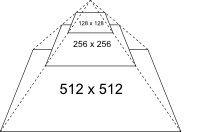
\includegraphics[scale=0.5]{figures/resolution_pyramid.png}
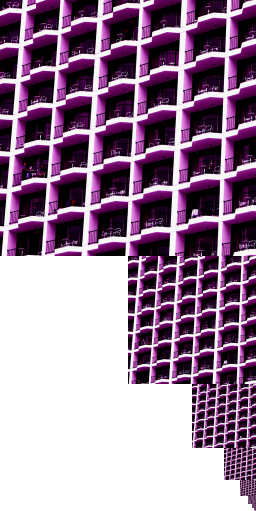
\includegraphics[scale=0.5]{figures/texture_mipmap_256.png}

\subsubsection{Mip-Mapping in OpenGL}

\begin{itemize}
	\item Um eine Mipmap zu verwenden, müssen folgende Parameter gesetzt werden:
	\begin{lstlisting}
glTexParameteri(
	GL_TEXTURE_2D,
	GL_TEXTURE_MAG_FILTER,
	GL_LINEAR
);
glTexParameteri(
	GL_TEXTURE_2D,
	GL_TEXTURE_MIN_FILTER,
	GL_LINEAR_MIPMAP_LINEAR
);
glTexParameteri(
	GL_TEXTURE_2D,
	GL_GENERATE_MIPMAP,
	GL_TRUE
);
glTexImage2D (...);
	\end{lstlisting}
	\item Mögliche Parameterwerte für den \textit{GL\_TEXTURE\_MIN\_FILTER} sind: \textit{GL\_NEAREST\_MIPMAP\_NEAREST, GL\_LINEAR\_MIPMAP\_NEAREST, GL\_NEAREST\_MIPMAP\_LINEAR, GL\_LINEAR\_MIPMAP\_LINEAR}
	\item Beim \textit{GL\_TEXTURE\_MAG\_FILTER} ist die Verwendung von Mipmaps nicht sinnvoll und wird auch nicht unterstützt
\end{itemize}

\subsubsection{Wirkung der Textur}

\begin{itemize}
	\item Mit der Funktion
	\begin{lstlisting}
glTexEnv(
	GL_TEXTURE_ENV,
	GL_TEXTURE_ENV_MODE,
	GL_REPLACE
);
	\end{lstlisting}
	kann beeinflusst werden, wie die Texturfarbe $C_s$ und der Alphakanal $A_s$ mit dem aktuellen Fragment (Farbwert $C_f$ und Alphakanal $A_f$) kombiniert wird
	\item Mögliche Parameter sind u.a \textit{GL\_REPLACE, GL\_MODULATE, GL\_DECAL, GL\_BLEND} oder \textit{GL\_ADD}
\end{itemize}

\begin{tabular}{|c|c|c|}
\hline 
 & \textit{GL\_RGB} & \textit{GL\_RGBA} \\ 
\hline 
\textit{GL\_REPLACE} & $C = C_s, A = A_f$ & $C = C_s, A = A_s$ \\ 
\hline 
\textit{GL\_MODULATE} & $C = C_f C_s, A = A_f$ & $C = C_f C_s, A = A_f A_f$ \\ 
\hline 
\textit{GL\_DECAL} & $C = C_s, A = A_f$ & $C = C_f(1 - A_s) + C_s A_s, A = A_f$ \\ 
\hline 
\textit{GL\_BLEND} & $C = C_f(1  C_s) + C_s C_s, A = A_f$ & $C = C_f(1 - C_s) + C_s C_s, A = A_f A_s$ \\ 
\hline 
\textit{GL\_ADD} & $C = C_f + C_s, A = A_f$ & $C = C_f + C_s, A = A_f A_s$ \\ 
\hline 
\end{tabular} 

\end{document}
